\documentclass[a4paper,12pt]{article}
\usepackage[utf8]{inputenc}
\usepackage[T1]{fontenc}
\usepackage[polish]{babel}
\usepackage{graphicx}
\usepackage{float}
\usepackage{geometry}
\usepackage{parskip}
\usepackage{tabularx} % Dodano do tabeli ryzyka
\usepackage{booktabs} % Dodano dla estetyki tabel
 \usepackage{hyperref}
\usepackage{pdfpages}
 \usepackage{amsmath}
 \usepackage{xcolor}
\usepackage{listings}
\geometry{
 a4paper,
 total={170mm,257mm},
 left=20mm,
 top=20mm,
}
% --- KONFIGURACJA KOLORÓW ---
\definecolor{codegreen}{rgb}{0,0.6,0}
\definecolor{codegray}{rgb}{0.5,0.5,0.5}
\definecolor{codepurple}{rgb}{0.58,0,0.82}
\definecolor{backcolor}{rgb}{0.95,0.95,0.92}
\definecolor{codeblue}{rgb}{0.1,0.1,0.8}

% --- GLOBALNE USTAWIENIA LISTINGÓW ---
\lstset{
    backgroundcolor=\color{backcolor},   % kolor tła
    commentstyle=\color{codegreen},      % kolor komentarzy
    keywordstyle=\color{codeblue}\bfseries, % kolor słów kluczowych
    numberstyle=\tiny\color{codegray},   % styl numerów linii
    stringstyle=\color{codepurple},      % styl dla tekstów (stringów)
    basicstyle=\ttfamily\small,          % monospaced czcionka dla kodu
    breakatwhitespace=false,             % łamanie linii tylko na białych znakach
    breaklines=true,                     % automatyczne zawijanie długich linii
    captionpos=b,                        % podpis na dole (b - bottom)
    keepspaces=true,                     % zachowanie wcięć i spacji
    numbers=left,                        % numery linii po lewej stronie
    numbersep=5pt,                       % odległość numerów od kodu
    showspaces=false,                    % nie pokazuj specjalnych znaczników spacji
    showstringspaces=false,              % nie pokazuj znaczników spacji w stringach
    showtabs=false,                      % nie pokazuj znaczników tabulacji
    tabsize=4,                           % szerokość tabulacji (4 spacje)
    frame=single,                        % ramka wokół kodu
    rulecolor=\color{codegray}           % kolor ramki
}

% --- SPECJALNA DEFINICJA DLA PLIKÓW .CONF ---
% Ponieważ 'listings' nie ma domyślnego języka ".conf", definiujemy własny prosty styl
\lstdefinelanguage{conf}{
    morecomment=[l]{\#},
    morestring=[b]",
    morestring=[b]',
    morekeywords={server, listen, server_name, root, index, location} % przykładowe słowa kluczowe (np. Nginx)
}

\title{Badanie skuteczności i implementacja rozwiązań w obronie przed różnymi technikami ataków DDoS - PDI 1}
\author{Artur Brogowicz }
\date{March 2026}

\begin{document}

\maketitle
\tableofcontents
\newpage

\section{Wprowadzenie}
\section{Analiza stanu wiedzy o najbardziej dotkliwych atakach DDoS}
Globalny rozwój i rosnąca powszechoność wykorzystywania architektur chmurowych połączony z postępem w implementacji sieci o coraz wyższych przepływnościach, jest przyczyną intensyfikacji zagrożeń związanych z rozproszonymi atakami odmowy usługi (ang. Distributed Denial of Service – DDoS). Dane analityczne wyraźnie wskazują na wykładniczy trend wzrostowy występowania tego typu zagrożeń. Jak wskazują zestawienia nowszych badań \cite{Detecting and Mitigating DDoS Attacks with AI: A Survey}, między styczniem 2020 roku a marcem 2021 roku odnotowano globalny wzrost liczby ataków o 55\%, co uległo przyśpieszeniu w kolejnych latach, osiągając przyrost na poziomie 75\% w pierwszej połowie 2022 roku. W związku z tym znacząco wzrosła wartość rynku zabezpieczeń i mitygacji DDoS, rynek wyceniono na 3.9 miliarda dolarów amerykańskich w 2022 roku, według prognoz osiągnie wartość ponad 7 miliardów dolarów do roku 2027. Ewolucja technik wykorzystywanych przez atakujących również postępuje, obserwowane jest wyraźne odejście od prostych prób wysycenia pasma sieciowego na rzecz wielowarstwowych wektorów ataków, operujących na asymetrii zasobów oraz uderzeniach wymierzonych w specyficzną i konkretną logikę warstwy aplikacyjnej. W obliczu tych wyzwań integracja nowoczesnych technik obronnych, w szczególności algorytmów uczących się na dużych zbiorach danych (ML), jest koniecznością dla utrzymania ciągłości działania systemów.
\subsection{Ataki wolumetryczne i sieciowe (L3 i L4)}
Ataki realizowane w warstwie sieciowej (L3) oraz transportowej (L4) modelu referencyjnego ISO/OSI stanowią podstawowy, lecz wciąż intensywnie rozwijany rdzeń operacji DDoS. Ich bezpośrednim celem jest wyczerpanie dostępnej przepustowości łączy telekomunikacyjnych prowadzących do atakowanej maszyny lub całkowite wysycenie skończonych zasobów sprzętowych urządzeń brzegowych, takich jak:
\begin{itemize}
    \item tablice stanów w zaporach sieciowych (ang. firewalls),
    \item bufory interfejsów routerów rdzeniowych,
    \item procesory sieciowe w urządzeniach takich jak routery, switche,
\end{itemize}  
Skuteczność tych wektorów ataku wynika z generowania gigantycznego wolumenu ruchu sieciowego, często przy użyciu rozproszonych sieci przejętych urządzeń - botnetów, które wykorzystują architektoniczne właściwości protokołów, takie jak bezstanowość UDP czy mechanikę alokacji pamięci i rezerwacji zasobów przy zestawianiu sesji TCP. Mitygacja tego typu zagrożeń wymaga implementacji zaawansowanych strategii inżynierii ruchu, w tym technik detekcji poza pasmem (ang. out-of-band) oraz infrastruktury o ogromnej przepustowości.
\subsubsection{SYN flood}
Atak typu SYN flood jest jednym z najbardziej klasycznych i fundamentalnych ataków, realizowany w warstwie transportowej L4, bezpośrednio wykorzystuje specyfikację protokołu Transmission Control Protocol - TCP. Aby w pełni zrozumieć działanie tego ataku, należy odnieść się do trójetapowego procesu nawiązywania połączenia (ang. three-way handshake), który w tym protokole jest wymagany do zainicjowania sesji komunikacyjnej między maszynami przez sieć. W typowych warunkach klient rozpoczyna nawiązywanie połączenia wysyłając do serwera segment TCP z ustawioną flagą SYN -Synchronize oraz wygenerowanym numerem sekwencyjnym. Po odebraniu takiego segmentu serwer docelowy alokuje odpowiednie zasoby w pamięci operacyjnej systemu, tworzony jest tzw. wpis w kolejce połączeń oczekujących, znanej jako SYN backlog queue. Następnie serwer docelowy odpowiada klientowi segmentem zawierającym flagi SYN i ACK (Acknowledgment). Segment ten zawiera również potwierdzenie odebranego numeru sekwencyjnego (w postaci zinkrementowania jego wartości go o 1) oraz nowy numer sekwencyjny wygenerowany przez serwer. W tym momencie połączenie na serwerze przechodzi w stan na wpół otwarty (ang. half-open connection). Ostatnim etapem jest odesłanie przez klienta finalnego segmentu ACK wraz z zinkrementowanymi wartościami numeru sekwencyjnego i potwierdzenia, po którego odebraniu serwer w pełni zestawia połączenie, zmieniając jego stan na ESTABLISHED. 
\begin{figure}[H]
    \centering
    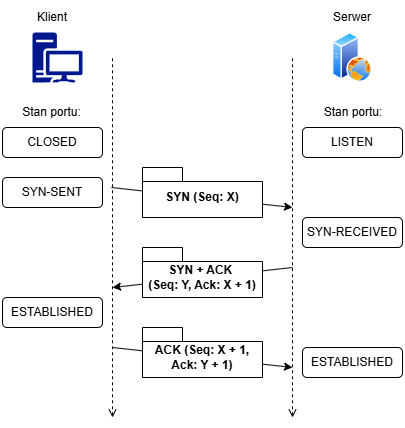
\includegraphics[width=0.5\linewidth]{images/TCP-3-way-handshake.png}
    \caption{Schemat ustanawiania sesji w protokole TCP (tzw. 3-way handshake) z uwzględnieniem wymiany segmentów i zmian stanów portów. \\ Źródło: Opracowanie własne na podstawie standardu RFC 793.}
    \label{fig:placeholder}
\end{figure}
Istotą ataku SYN flood jest masowe generowanie segmentów SYN, w których adresy źródłowe IP są fałszowane (ang. IP spoofing). Serwer ofiary, postępując zgodnie ze standardem RFC dla protokołu TCP, dla każdego z tych sfałszowanych żądań alokuje cenne zasoby w kolejce backlog i odsyła segment SYN$+$ACK pod wcześniej otrzymany adres IP, po czym przechodzi w stan oczekiwania. Oczekiwany finalny segment ACK od złośliwego klienta nigdy nie nadchodzi, co powoduje, że serwer utrzymuje te na wpół otwarte połączenia aż do momentu upłynięcia określonego limitu czasu (ang. timeout). Ze względu na skończoną wielkość kolejki połączeń oczekujących, ciągły napływ sfałszowanych segmentów SYN prowadzi do jej natychmiastowego przepełnienia. W konsekwencji system operacyjny ofiary zaczyna bezwarunkowo odrzucać nowe żądania nawiązania połączenia od prawdziwych użytkowników, co realizuje skutkuje odmową dostępu do usługi. Dodatkowo mechanizm ten tworzy pole do pokrewnych złośliwych technik, takich jak przechwytywanie sesji TCP (ang. TCP session hijacking), gdzie napastnik próbuje nieuprawnienie wstrzyknąć segmenty protokołu transportowego w strumień wymieniany w autoryzowanym połączeniu między ofiarą a systemem zaufanym.

W ramach przeciwdziałania temu atakowi bez konieczności nieustannej rozbudowy zasobów sprzętowych serwera, został opracowany mechanizm obronny ciasteczek SYN (ang. SYN cookies). Została zaprojektowana w 1996 roku przez Daniela J. Bernsteina. Ta koncepcja polega na rezygnacji z alokacji zasobów na serwerze po odebraniu segmentu ACK od klienta, nie jest tworzony wpis w kolejce backlogu. Zamiast tego serwer po odebraniu segmentu inicjującego generuje unikalną wartość kryptograficzną, która jest odsyłana do klienta jako początkowy numer sekwencyjny w segmencie SYN$+$ACK. W konsekwencji następuje przeniesienie stanu połączenia z pamięci serwera do samego pakietu sieciowego, jednak mechanizm ten zaczyna działać dopiero gdy serwer ma włączone ciasteczka SYN oraz jego kolejce SYN.

Ciasteczko ma rozmiar 32 bitów, jego struktura jest jasno zdefiniowana, składa się z poniższych elementów:
\begin{itemize}
    \item 5 bitów znacznika czasu (ang. timestamp), którego wartość inkrementuje się co kilkadziesiąt sekund aby zapobiec atakamom powtórzeniowym.
    \item 3 bity znacznika reprezentującego zakodowaną wartość maksymalnej długości segmentu (Maximum Segment Size) zadeklarowanej przez klienta w pierwotnym żądaniu.
    \item 24 bity przyciętego skrótu kryptograficznego obliczanego funkcją skrótu na podstawie następujących parametrów połączenia:
    \begin{itemize}
        \item Adres IP klienta
        \item Adres IP serwera
        \item Port klienta
        \item Port serwera
        \item Czas t
        \item Klucz znany wyłącznie serwerowi generowany losowo przy starcie systemu
    \end{itemize}
\end{itemize}
Wartość ciasteczka C można zapisać następująco:
$$C = \text{Timestamp} \parallel \text{MSS}_{index} \parallel \text{Hash}(IP_{src}, IP_{dst}, P_{src}, P_{dst}, \text{Timestamp}, K_{secret})$$
gdzie operator $\parallel$ oznacza konkatenację bitową, a $K_{secret}$ jest tajnym kluczem serwera.

W przypadku autentycznego żądania SYN klienta, po odebraniu SYN$+$ACK klient odpowie finalnym segmentem ACK w którym numer potwierdzenia (ang. Acknowledgment Number) będzie równy wartości otrzymanego ciasteczka powiększonej o jeden. Po odebraniu tego segmentu serwer dekoduje numer potwierdzenia, weryfikuje poprawność 24-bitowego skrótu kryptograficznego oraz odtwarza pierwotną wartość MSS. Zasoby w pamięci serwera rezerwowane są zatem wyłącznie dla połączeń, które pomyślnie przeszły weryfikację kryptograficzną, co sprawia, że atak SYN flood oparty na fałszowaniu IP staje się nieskuteczny - nie dochodzi do wyczerpania pamięci po stronie serwera. 

Analizując ten mechanizm należy jednak wspomnieć również o jego wadach. W oryginalnej implementacji ciasteczek SYN kodowanie informacji na 32 bitach uniemożliwia zapisanie ważnych opcji TCP, które standardowo są negocjowane w segmencie SYN np. skalowanie okna (ang. window scaling) czy SACK dla niestabilnych łącz. Obecny jest również narzut obliczeniowy obciążający dodatkowo jednostkę CPU, wynikający z obliczania kryptograficznego skrótu dla każdego segmentu SYN. 

Aby zniwelować problem utraty opcjonalnych parametrów połączenia, współczesne implementacje m.in. jądro systemu Linux wprowadzają rozwiązanie polegające na wykorzystaniu opcji znaczników czasu protokołu TCP (ang. TCP Timestamps), zdefiniowanej w RFC 1323. Mechanizm znaczników czasu opiera się na tym, że host wysyłający segment umieszcza w nim swój aktualny czas w polu TSval (Timestamp Value), a odbiorca w odpowiedzi ma obowiązek odesłać tę samą wartość w polu TSecr (Timestamp Echo Reply), nie analizując jej zawartości.

W sytuacji, gdy serwer znajduje się pod atakiem SYN Flood i są aktywne ciasteczka SYN, serwer sprawdza czy klient w żądaniu SYN zadeklarował obsługę opcji Timestamps. Jeśli tak, serwer nie zapisuje w swoim segmencie SYN$+$ACK rzeczywistego czasu. Zamiast tego modyfikuje 32-bitowe pole TSval, w którym koduje brakujące parametry na podstawie wartości wskazanych w pierwszym segmencie SYN od klienta. Struktura tego zmodyfikowanego znacznika czasu w systemie Linux przedstawia się następująco:
\begin{itemize}
\item Najbardziej znaczące 26 bitów: dostosowany rzeczywisty znacznik czasu, pozwala on na zachowanie zgodności z mechanizmem PAWS (Protection Against Wrapped Sequences).
\item 1 bit: flaga obsługi ECN (Explicit Congestion Notification).
\item 1 bit: flaga obsługi SACK (Selective Acknowledgment).
\item Najmniej znaczące 4 bity: zadeklarowana przez klienta wartość skalowania okna (Window Scaling), podawany jako przesunięcie bitowe (potęga liczby 2 w zakresie od 0 do 14).
\end{itemize}
Gdy autentyczny klient odsyła finalny segment ACK, bezpośrednio jest kopiowana wartość z TSval serwera do własnego pola TSecr. Serwer, po pomyślnej weryfikacji głównego 32-bitowego ciasteczka SYN, wyodrębnia za pomocą masek bitowych informacje zakodowane w TSecr. Dzięki temu procesowi serwer odzyskuje wszystkie niezbędne parametry, co pozwala na ostateczne ustanowienie w pełni zoptymalizowanego połączenia bez konieczności alokowania pamięci dla stanów na wpół otwartych.
\subsubsection{UDP flood}
W tym ataku wykorzystywany jest bezstanowy protokół transportowy UDP oparty na datagramach. W przeciwieństwie do połączeniowego protokołu TCP, nie wymaga on wymiany komunikatów inicjujących ani potwierdzania odbioru poszczególnych pakietów przez strony komunikacji, co czyni go idealnym narzędziem w rękach napastników dążących do wygenerowania gigantycznego wolumenu danych przy absolutnie minimalnym nakładzie pracy oraz mocy obliczeniowej po stronie kontrolowanego botnetu. Atak UDP flood wykorzystuje znaczącą asymetrię, polegając na zasypywaniu systemu docelowego masową liczbą stosunkowo małych datagramów UDP, najczęściej ze sfałszowanymi adresami źródłowymi IP, które są kierowane na całkowicie losowe porty urządzenia ofiary. 

Problematyczny jest również fakt, iż kiedy system operacyjny stacji docelowej, routera lub urządzenia brzegowego odbiera datagram UDP, standardowa procedura obsługi stosu sieciowego wymaga sprawdzenia, czy do wskazanego portu docelowego przypisana jest jakakolwiek aktywna usługa, która nasłuchuje połączenia (ang. listening state). W przypadku ataku skierowanego na losowe numery portów, prawdopodobieństwo trafienia na aktywną usługę jest znikome. W takiej sytuacji, zgodnie ze standardami zachowania w sieci IP, urządzenie docelowe jest zobligowane do wygenerowania i odesłania komunikatu błędu ICMP Destination Unreachable pod adres źródłowy wskazany w złośliwym pakiecie. Ten proces oddziałuje w sposób zdecydowanie negatywny na wydajność systemu serwera na dwóch płaszczyznach. Po pierwsze, interfejsy sieciowe ofiary zapychane są ogromną liczbą nadchodzących datagramów. Po drugie, zasoby jednostki CPU są wykorzystywane do nieustannej weryfikacji tablicy portów i generowania pakietów ICMP.

\begin{figure}[H]
    \centering
    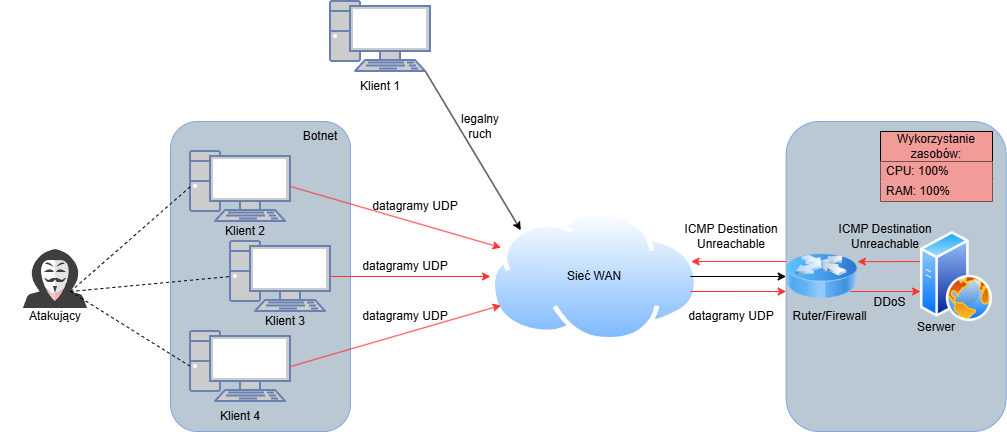
\includegraphics[width=1\linewidth]{images/UDP-flood.png}
    \caption{Schemat przebiegu ataku wolumetrycznego typu UDP flood z uwzględnieniem generowania komunikatów ICMP oraz wyczerpania zasobów serwera ofiary. \\ Źródło: Opracowanie własne.}
    \label{fig:placeholder}
\end{figure}

W związku z bezstanowością protokołu UDP, proces odróżniania pakietów złośliwych od legalnego ruchu aplikacyjnego za pomocą tradycyjnych zapór sieciowych czy systemów IPS jest również podatny na przeciążenia. Głęboka inspekcja pakietów (ang. Deep Packet Inspection) każdego pakietu przy wieloterabitowych atakach przekracza możliwości obliczeniowe specjalizowanych układów scalonych urządzeń przetwarzających ruch sieciowy \cite{DDoS Protection and Mitigation: A 2026 Guide to Defending Modern Networks}. 

Najnowsze rozwiązania cyberbezpieczeństwa kładą nacisk na analizę przepływów (ang. flow-based detection) oraz architekturę poza głównym pamem (ang. out-of-band), gdzie urządzenie monitorujące wykonuje kopię całego ruchu sieciowego i wysyła ją do systemu analitycznego. Analiza przepływów polega na ekstrakcji kluczowych cech pakietów do grupowania w ramach przepływów. W standardzie NetFlow ekstrachowane są następujące parametry \label{Netflow}:
\begin{itemize}
    \item źródłowy adres IP,
    \item docelowy adres IP,
    \item źródłowy numer portu,
    \item docelowy numer portu,
    \item protokół,
\end{itemize}
Następnie analizowane są kluczowe statystyki opisujące komunikację: adresy, porty, liczbę pakietów na sekundę (pps) i bitów na sekundę (bps) oraz wielkości pakietów. Informacje te są następnie wprowadzane do rozproszonych systemów analitycznych typu Big Data, gdzie algorytmy profilowania zachowań tworzą dynamiczne linie bazowe (ang. dynamic baselining) dla każdego prefiksu IP, a przy użyciu uczenia maszynowego wykrywają odchylenia charakterystyczne dla wolumetrycznych powodzi UDP. Automatyzacja reakcji po detekcji ataku może polegać na wykorzystaniu protokołu sterowania trasami z poziomu sieci międzyoperatorskich BGP, np. BGP Flowspec do odfiltrowania złośliwych portów, lub przekierowaniu złośliwego ruchu do chmurowych centrów czyszczących (ang. Scrubbing Centers) \cite{DDoS Protection and Mitigation: A 2026 Guide to Defending Modern Networks}.
\subsubsection{DNS Amplification}
Atak DNS Amplification bazuje na zjawisku odbicia (ang. reflection) oraz zjawisku wzmocnienia (ang. amplification). Odbicie polega na skierowaniu odpowiedzi serwera do ofiary poprzez sfałszowanie źródłowego adresu IP w pierwotnym zapytaniu wysyłanym przez atakującego. Wzmocnienie wynika z uzyskania nieproporcjonalnie większej odpowiedzi do maszyny ofiary niż rozmiar wysyłanego pierwotnie żądania. Jest to jeden z najbardziej skutecznych ataków wolumetrycznych, wykorzystujący dysproporcję w konsumpcji przepustowości pomiędzy maszyną inicjującą a infrastrukturą ofiary, eksploatując fundamentalne właściwości protokołu Systemu Nazw Domenowych (DNS).W szczególności podatne są otwarte serwery rekursywne (ang. open resolvers), które odpowiadają na zapytania od dowolnego adresu w sieci publicznej.

Atak DNS Amplification można opisać w poniższych krokach \cite{DNS amplification attack}:
\begin{enumerate}
    \item Host należący do botnetu generuje datagram UDP z zapytaniem DNS ze sfałszowanym źródłowym adresem IP w nagłówku protokołu IP, wstawiony jest adres IP hosta ofiary. 
    \item Zapytanie jest zbudowane w taki sposób, aby uzyskać odpowiedź z serwera DNS o maksymalnym rozmiarze. Nagłówek zapytania operuje często na specjalnym argumencie/typie rekordu ANY lub TXT, wymuszając na serwerze zrzut wszystkich dostępnych informacji powiązanych ze strefą. Kluczowe jest tu również wykorzystanie mechanizmu EDNS0 (ang. Extension Mechanisms for DNS), który pozwala na zwiększenie limitu wielkości pakietu UDP z klasycznych 512 bajtów do nawet 4096 bajtów.
    \item Podatny serwer DNS traktuje zapytanie jako autentyczne, ponieważ nie ma mechanizmów uwierzytelniających w podstawowym UDP i przygotowuje pakiet odpowiedzi o rozmiarze wielokrotnie większym od rozmiaru zapytania.
    \item Wielokrotnie powiększona odpowiedź jest odsyłana pod sfałszowany adres źródłowy. W efekcie ofiara ataku otrzymuje lawinę nieżądanych danych, co w konsekwencji prowadzi do wysycenia jej brzegowych punktów styku z Internetem i niedostępności usługi.
\end{enumerate}
\begin{figure}[H]
    \centering
    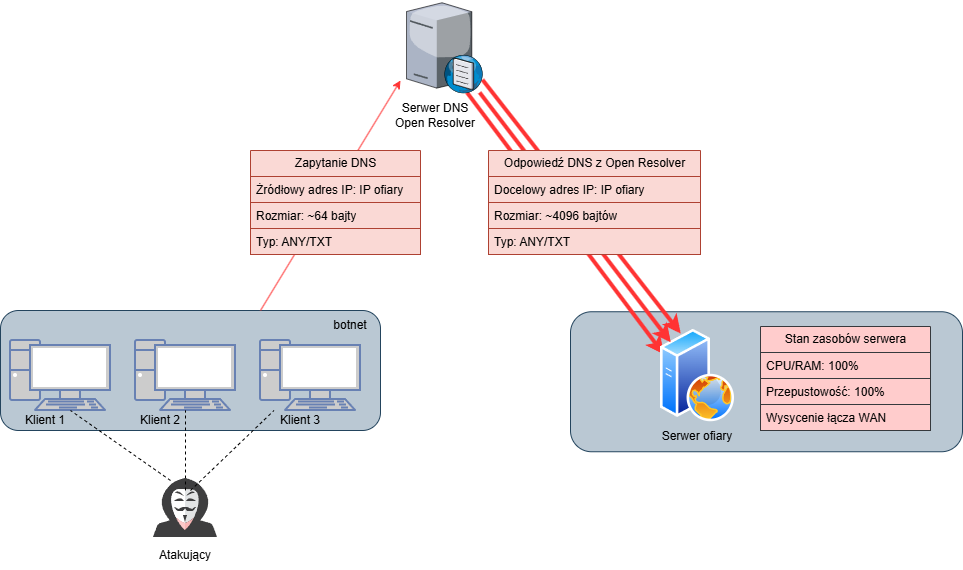
\includegraphics[width=1\linewidth]{images/DNS-Amplification.png}
    \caption{Schemat przebiegu ataku wolumetrycznego typu DNS Amplification z uwzględnieniem zjawiska spoofingu, odbicia oraz wzmocnienia odpowiedzi. \\ Źródło: Opracowanie własne.}
    \label{fig:dns_amplification}
\end{figure}
Mitygacja ataków amplifikacyjnych odbywa się na wielu równoległych płaszczyznach struktury sieciowej. Jednym z mechanizmów obronnych jest filtrowanie wejściowe (ang. Ingress Filtering), wdrażane po stronie dostawcy usług internetowych (ang. Internet Service Provider), polegający na natychmiastowym zrzucaniu pakietów wychodzących z ich infrastruktury, których źródłowe adresy IP nie należą do zarządzanej przez nich przestrzeni adresowej, co bezpośrednio uniemożliwia IP spoofing. Na poziomie serwerów domenowych wdraża się zaawansowane limity szybkości, znane jako RRL (ang. Response Rate Limiting), które radykalnie ograniczają liczbę jednakowych odpowiedzi odsyłanych do pojedynczego docelowego adresu IP w jednostce czasu. Dla skali produkcyjnej skutecznym rozwiązaniem jest integracja globalnych architektur Anycast zarządzanych przez liderów usług chmurowych. Przykładem może być system Gatebot wdrożony w chmurze Cloudflare, gdzie cały wolumen odbitych danych jest rozpraszany i absorbowany przez tysiące centrów danych, co zapobiega blokadzie pojedynczego serwera ofiary.
\subsection{Ataki niewolumetryczne w warstwie aplikacyjnej (L7)}
Ataki w warstwie aplikacyjnej modelu ISO/OSI (L7), w przeciwieństwie do wcześniej omówionych metod wolumetrycznych, charakteryzują się precyzyjnym podejściem do powolnego i metodycznego konsumowania zasobów serwera ofiary (ang. "low and slow"). Ich celem nie jest wysycenie przepustowości pasma telekomunikacyjnego, lecz asymetryczne wyczerpanie ograniczonych zasobów przetwarzania po stronie samego systemu operacyjnego lub serwera aplikacji takich jak:
\begin{itemize}
    \item pule dostępnych połączeń,
    \item wątki robocze procesora,
    \item dostępna pamięć alokowana do utrzymywania sesji użytkowników.
\end{itemize}
W związku z tym, że złośliwy ruch sieciowy generowany przez atakujących w pełni naśladuje poprawne sesje TCP i żądania HTTPS, podstawowe metody detekcyjne oparte na sygnaturach nie spełniają skutecznie swojej roli.
\subsubsection{SlowLoris}
Ten precyzyjny wektor ataku został zaprezentowany publicznie w 2009 roku przez inżyniera Roberta Hansena jako narzędzie koncepcyjne (ang. proof-of-concept). Od tego czasu stał się wzorcem klasy ataków skierowanych na serwery WWW. Atak celuje bezpośrednio w serwery wielowątkowe, które zawsze posiadają granicę maksymalnej liczby równolegle obsługiwanych klientów. Wykorzystywany jest mechanizm protokołu HTTP, konkretnie znacznik podwójnego załamania linii "\verb|\r\n\r\n|" w żądaniach HTTP GET, który sygnalizuje serwerowi zakończenie żądania. Atak typu SlowLoris jest realizowany w następujących krokach \cite{Slowloris DDoS attack}:
\begin{enumerate}
    \item Atakujący otwiera wiele (tysiące) prawidłowych połączeń TCP do serwera docelowego, a następnie rozpoczyna wysyłanie spreparowanych, niepełnych nagłówków żądania HTTP, w których celowo pomija końcowy ciąg "\verb|\r\n\r\n|"
    \item Serwer ofiary dla każdego z przychodzących żądań jest zmuszony do alokacji odzielnego wątku w pamieci operacyjnej, ponieważ żądania wysyłane przez atakującego są poprawnie zbudowane.
    \item Atakujący nie pozwala serwerowi również na zerwanie połączenia z powodu bezczynności - sesje w których nie ma wymiany ruchu sieciowego. Wykorzystywane są narzędzia do wysyłania małych fragmentów danych nagłówkowych w regularnych odstępach czasu. W konsekwencji resetowane są liczniki czasu bezczynności (timeout) a wszystkie połączenia atakującego są podtrzymywane przy życiu i obsługiwane przez serwer.
    \item Proces ten doprowadza do sytuacji, w której docelowy serwer WWW zostaje zmuszony do nieskończonego utrzymywania otwartych połączeń. W rezultacie szybko zostaje wyczerpana pula dostępnych wątków, po czym aplikacja staje się niedostępna dla żądań od uprawnionych użytkowników z zewnątrz.
\end{enumerate}
\begin{figure}[H]
    \centering
    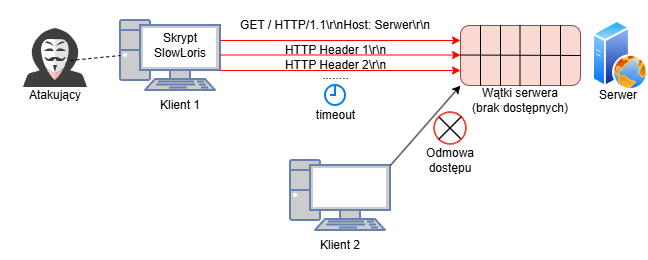
\includegraphics[width=0.8\linewidth]{images/SlowLoris.png}
    \caption{Schemat wektora ataku SlowLoris obrazujący powolne wysyłanie niepełnych żądań HTTP i asymetryczne wyczerpanie puli wątków serwera WWW \\ Źródło: Opracowanie własne}
    \label{fig:slowloris}
\end{figure}
Ponieważ atak operuje na zestawionych i stabilnych sesjach TCP, podstawowym narzędziem obronnym jest konfiguracja dostatecznie krótkiego czasu timeout dla procesu parsowania nagłówków na serwerze. Jest to problematyczne rozwiązanie, ponieważ ustawienie zbyt krótkiego czasu timeout powoduje rozłączanie sesji legalnych użytkowników z niestabilnym i wolnym łączem sieciowym. Skuteczniejszą obroną przed atakiem SlowLoris jest zastosowanie pośrednich serwerów typu reverse proxy z funkcją równoważenia obciążenia (ang. load balancing) oraz mechanizmami pamięci podręcznej (ang. cache). Rozwiązanie to już na poziomie architektonicznym pozwala obsługiwać tysiące powolnych połączeń bez dedykowania im osobnych wątków systemowych właściwego serwera. Współcześnie najczęściej wykorzystywane są do tego zadania maszyny z zasobów chmurowych pełniących również funkcje WAF i wymuszających limity wywołań w czasie dla poszczególnych klientów. \cite{Slowloris attack}
\subsubsection{R.U.D.Y}
R.U.D.Y - ang. Are You Dead Yet, atak jest bezpośrednio powiązany z wcześniej omówionym atakiem SlowLoris, również w tym przypadku dochodzi do powolnego i konsekwentnego zużywania zasobów serwera ofiary, prowadząc do niedostępności działającej usługi. Różnica między tymi wektorami ataków jest na poziomie mechaniki protokołu HTTP, R.U.D.Y wykorzystuje żądania HTTP POST stosowane m.in. do przesyłania danych w formularzach internetowych oraz przesyłania plików. 

W prawidłowym żądaniu HTTP POST, w sekcji zdefiniowanych nagłówków, klient przekazuje parametr Content-Length, informujący serwer o fizycznym rozmiarze w bajtach ciała przesyłanej wiadomości. Pozwala to systemowi docelowemu na prawidłową inicjalizację strumienia bufora oczekującego na dane. Mechanizm R.U.D.Y. rozpoczyna się od poprawnego sformułowania i otwarcia połączenia aplikacyjnego z formularzem. W nagłówkach żądania POST atakujący wprowadza zawyżoną wartość dla atrybutu Content-Length, sugerując przesłanie do systemu znaczącej paczki danych rzędu megabajtów. Po poprawnym zamknięciu bloku nagłówków ciągiem "\verb|\r\n\r\n|", atak przechodzi do fazy przesyłania ciała żądania (ang. payload). Aby utrzymać aktywne połączenie z serwerem jak najdłużej, atakujący przesyła dane z niską szybkością transferu. W rezultacie, szczególnie przy użyciu sieci botnet do przeprowadzenia ataku na dużą skalę, zasoby po stronie serwera zostają skonsumowane do obsługi żądań atakującego i stają się niedostępne dla legalnych użytkowników usługi.
\begin{figure}[H]
    \centering
    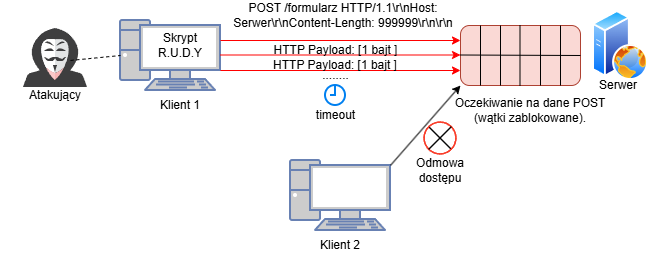
\includegraphics[width=0.8\linewidth]{images/RUDY.png}
    \caption{Schemat ataku R.U.D.Y. obrazujący manipulację nagłówkiem Content-Length oraz powolne przesyłanie ciała żądania HTTP POST w celu wyczerpania wątków serwera \\ Źródło: Opracowanie własne}
    \label{fig:rudy_attack}
\end{figure}
Podobnie jak w przypadku ataku SlowLoris, mitygacja wektora R.U.D.Y. stanowi duże wyzwanie dla tradycyjnych systemów zabezpieczeń, takich jak zapory sieciowe warstwy L3/L4, ponieważ złośliwy ruch opiera się na technicznie poprawnych żądaniach HTTP i w pełni zestawionych sesjach TCP. Standardowe mechanizmy obronne oparte na limitach czasu bezczynności są nieskuteczne, ponieważ atakujący nieustannie transmituje fragmenty danych, tym samym podtrzymując aktywność połączenia.

Skuteczna obrona wymaga wdrożenia zaawansowanych mechanizmów inspekcji i kontroli bezpośrednio w warstwie aplikacyjnej (L7). Architektonicznym rozwiązaniem jest zastosowanie rewersyjnych serwerów pośredniczących lub systmeów WAF, tak jak w przypadku mitygacji ataku SlowLoris, skonfigurowanych w trybie buforowania żądań. W takiej konfiguracji serwer pośredniczący samodzielnie przyjmuje i kompletuje całe ciało wiadomości POST od klienta. Żądanie jest przekazywane do właściwego serwera aplikacyjnego gdy zostanie odebrany od klienta ostatni zadeklarowany bajt w nagłówku Content-Length. Dzięki temu serwer docelowy otrzymuje wyłącznie kompletne, gotowe do przetworzenia pakiety danych, a jego pula wątków roboczych jest chroniona przed zablokowaniem. Uzupełnieniem obrony strukturalnej jest wdrożenie rygorystycznych polityk dotyczących przepływu danych. Jeśli klient przesyła dane z szybkością poniżej ustalonego progu w charakterystyczny, regularny sposób lub sesja przekroczy globalny limit czasu, połączenie z serwerem jest przerywane. Współczesne chmurowe systemy WAF wzbogacają te metody o analizę behawioralną, potrafiąc rozpoznać anomalie w tempie interakcji z formularzami webowymi i odróżnić powolny atak DoS od użytkownika mobilnego ze słabym zasięgiem. \cite{Generator of Slow Denial-of-Service Cyber Attacks}
\subsubsection{HTTP/2 Rapid Reset}
Wprowadzenie standardu HTTP/2 znacząco zoptymalizowało przesyłanie zasobów webowych, głównie poprzez rozwiązanie problemu blokowania linii żądań (ang. head-of-line blocking), charakterystycznego dla protokołu HTTP/1.1. Innowacją w HTTP/2 było wdrożenie binarnego multipleksowania współbieżnych strumieni (ang. stream concurrency). Pozwala ono klientowi na wysyłanie wielu niezależnych żądań i asynchroniczne odbieranie odpowiedzi w ramach pojedynczego, ciągłego połączenia TCP. W sierpniu 2023 roku zidentyfikowano i masowo wykorzystano krytyczną podatność CVE-2023-44487, znaną jako Rapid Reset, bazującą na fundamentalnym błędzie projektowym specyfikacji tego protokołu. \cite{CVE-2023-44487}
Aby zapobiec wyczerpaniu zasobów serwera, specyfikacja HTTP/2 definiuje mechanizm negocjacji za pomocą ramki SETTINGS. Ustala ona maksymalny limit jednoczesnych strumieni. Jednocześnie protokół dopuszcza możliwość przerwania zainicjowanego żądania poprzez przesłanie ramki RST\_STREAM. Otrzymanie takiego komunikatu obliguje serwer do przerwania przetwarzania danego strumienia i natychmiastowej dealokacji przydzielonych mu zasobów pamięciowych.

Algorytm ataku Rapid Reset polega na metodycznym nadużywaniu mechanizmu zestawiania i przerywania strumieni. W ramach pojedynczego połączenia TCP atakujący generuje setki ramek inicjujących zapytania, po czym natychmiast przesyła odpowiadające im ramki RST\_STREAM. Ponieważ zresetowane strumienie natychmiast przestają wliczać się do limitu współbieżnych strumieni określonych w parametrze SETTINGS, system obronny nie przerywa połączenia TCP. Atakujący precyzyjnie nie przekracza ustalonego progu np. 100 aktywnych zapytań w danym momencie. Serwer aplikacyjny ofiary jest zmuszony do nieustannego rezerwowania zasobów na parsowanie nowych zapytań, alokację struktur danych i natychmiastowe wykonywanie procedur ich niszczenia. Ten proces generuje potężny narzut operacyjny po stronie serwera, prowadząc do błyskawicznego wyczerpania zasobów CPU (odmowa usługi), przy minimalnym wykorzystaniu przepustowości sieciowej przez botnet atakującego. \cite{HTTP/2 Rapid Reset: deconstructing the record-breaking attack}
\begin{figure}[H]
    \centering
    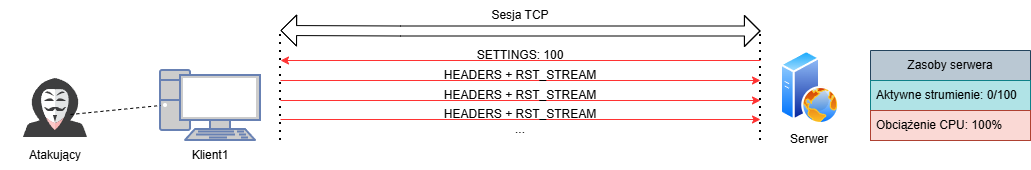
\includegraphics[width=1\linewidth]{images/HTTP2-Rapid-Reset.png}
    \caption{Schemat mechaniki ataku HTTP/2 Rapid Reset ukazujący omijanie limitu ramki SETTINGS poprzez anulowanie strumieni komunikatem RST\_STREAM oraz wynikające z tego wyczerpanie zasobów procesora \\ Źródło: Opracowanie własne}
    \label{fig:rapid_reset}
\end{figure}
Mitygacja ataku Rapid Reset w przeszłości wymagała aktualizacji na poziomie kodu źródłowego silników serwerów webowych oraz rekonfiguracji systemów WAF. Próby obniżenia w ramce SETTINGS limitu współbieżnych strumieni skutkowały problemami z niesłusznym blokowaniem legalnych użytkowników, których nowoczesne przeglądarki naturalnie generują duże pakiety asynchronicznych zapytań przy wczytywaniu złożonych interfejsów graficznych. 

Skutecznym podejściem w mitygacji tego ataku jest zastosowanie głębokiej analizy heurystycznej zliczającej częstotliwość występowania komunikatów RST\_STREAM w jednostce czasu dla danej sesji TCP. Jeśli klient przekracza dopuszczalne wzorce behawioralne, jego adres IP jest natychmiast blokowany, zrywając komunikację na poziomie warstwy transportowej. Dodatkowo konieczne są usprawnienia w planistach przetwarzania zadań (ang. dispatch code scheduling), aby zredukować narzut obliczeniowy generowany przez procesy alokacji i dealokacji nieukończonych zapytań. \cite{DDoS Protection and Mitigation: A 2026 Guide to Defending Modern Networks}
\subsection{Ataki wielowektorowe}
\subsubsection{Carpet Bombing}
Atak typu \textit{Carpet Bombing} stanowi zaawansowany wariant wolumetrycznych wektorów DDoS w warstwie sieciowej L3 i transportowej L4. Zjawisko to opiera się na celowym rozproszeniu złośliwego ruchu w celu ominięcia tradycyjnych mechanizmów detekcyjnych. Klasyczne ataki DDoS charakteryzują się wysoką koncentracją ruchu kierowanego na pojedynczy docelowy adres IP. Umożliwia to stosunkowo łatwą mitygację za pomocą statycznych limitów przepustowości przypisanych do konkretnego hosta, gdzie jednorazowe przekroczenie ustalonego progu automatycznie wyzwala procedury obronne dostawcy usług internetowych.

Architektura ataku \textit{Carpet Bombing} jest wektorem asymetrycznym, zaprojektowanym do eksploatacji ograniczeń tego modelu bezpieczeństwa. Zamiast obciążać pojedynczy cel, rozległe botnety równomiernie dystrybuują ruch na całe bloki adresacyjne CIDR w ramach wspólnych prefiksów trasowania BGP. 

Skuteczność tej metody opiera się na rozproszeniu wolumenu ataku poniżej progów detekcyjnych. Przykładowo, atak o łącznej przepustowości 200 Gbps, równomiernie rozłożony na 2000 docelowych adresów IP, generuje obciążenie rzędu zaledwie 100 Mbps dla każdego pojedynczego hosta. Dla lokalnych zapór sieciowych i statycznych filtrów sprzętowych taki przyrost ruchu bywa nieodróżnialny od standardowych fluktuacji, co zapobiega wyzwoleniu systemów prewencji. Natomiast w punktach agregacji takich jak główne routery krawędziowe i łącza dystrybucyjne w rdzeniu sieci ISP następuje skumulowanie pełnej skali przepływu 200 Gbps. Prowadzi to do całkowitego wyczerpania przepustowości infrastruktury operatora i dramatycznej degradacji usług dla wszystkich klientów w danym segmencie.\cite{Carpet-bombing Attacks Highlight the Need for Intelligent and Automated DDoS Protection}.

Złożone ataki wielowektorowe wykazały nieskuteczność tradycyjnych zapór sieciowych. Wyznaczyło to kierunek rozwoju w stronę analityki hybrydowej, bazującej na analizie strumieniowej (ang. Flow-based analytics), orkiestracji polityk BGP oraz chmurowych centrach mitygacji (ang. Scrubbing Centers). W klasycznym podejściu analiza inline generowała nadmierne obciążenie zasobów obliczeniowych na urządzeniach brzegowych. Współczesne mechanizmy mitygacyjne wykorzystują architekturę Big Data, która asynchronicznie agreguje zminimalizowane logi telemetryczne pochodzące z protokołów takich jak NetFlow, IPFIX czy sFlow. Zebrane dane są korelowane z informacjami z protokołu BGP, co pozwala na precyzyjne mapowanie źródeł ruchu i systemów autonomicznych ASN. Zgromadzona telemetria stanowi wejście dla algorytmów uczenia maszynowego, które wyznaczają dynamiczne linie bazowe dla obsługiwanego ruchu. Poprzez estymację entropii, modele te potrafią błyskawicznie zidentyfikować anomalie podsieciowe charakteryzujące się rozproszonym wolumenem typowym dla ataków Carpet Bombing, minimalizując jednocześnie odsetek fałszywie dodatnich blokad (ang. false positives) na wczesnym etapie narastania obciążenia.

W przypadku klasycznych ataków wolumetrycznych kierowanych na pojedynczy adres IP, operatorzy powszechnie stosowali metodę RTBH (ang. Remotely Triggered Black Hole). Mechanizm ten polega na rozgłoszeniu w sieci BGP zainfekowanego prefiksu z dedykowanym atrybutem społeczności, najczęściej oznaczanym wartością 666. Powoduje to wymuszenie na routerach brzegowych bezwarunkowego przekierowania całego ruchu skierowanego na dany adres do interfejsu zerowego null0. O ile RTBH z powodzeniem zapobiega saturacji łączy operatora, o tyle jego użycie skutkuje całkowitym odcięciem atakowanego hosta od legalnego ruchu, co oznacza zrealizowanie celu atakującego. Zastosowanie mechanizmu RTBH do całej podsieci podczas ataku Carpet Bombing przyniosłoby katastrofalne skutki, prowadząc do masowej niedostępności usług dla wszystkich klientów w danej puli adresowej.

Rozwiązaniem jest wdrożenie mechanizmu BGP FlowSpec (ang. BGP Flow Specifications), ustandaryzowanego w dokumentach RFC 5575 oraz RFC 8955 \cite{The ultimate weapon against DDoS — BGP Flowspec}. Technologia ta pozwala rozproszonej architekturze sieciowej na odejście od binarnych blokad całych adresów IP na rzecz propagowania reguł i sygnatur ataku. Filtry FlowSpec mogą uwzględniać kombinacje takich parametrów jak: 
\begin{itemize}
    \item port źródłowy,
    \item port docelowy,
    \item rozmiar nagłówka,
    \item typ protokołu warstwy transportowej - TCP/UDP,
    \item typ fragmentacji pakietu.
\end{itemize} 
Informacje te są propagowane w szkieletowej sieci operatorskiej poprzez komunikaty \textit{UPDATE} jako atrybut \textit{FLOW\_SPEC\_NLRI} (ang. Network Layer Reachability Information). Towarzyszą im akcje decyzyjne zdefiniowane w społecznościach rozszerzonych (ang. Extended Communities) w obrębie instancji VRF (ang. Virtual Routing and Forwarding). Dzięki orkiestracji polityk narzędziami analitycznymi, routery brzegowe odrzucają wyłącznie złośliwe pakiety należące do wektora ataku, zachowując pełną dostępność usług dla pożądanego ruchu.

\section{Analiza stanu wiedzy o metodach obrony przed atakami DDoS}
Skala współczesnych ataków rozproszonej odmowy usługi DDoS z roku na rok osiąga rekordowe wartości. Według danych dostawcy usług chmurowych Cloudflare, współczesne botnety generują ruch o wolumenie przekraczającym 3,8 Tbps oraz 2 miliardy pakietów na sekundę Bpps na poziomie warstwy sieciowej, a w przypadku ataków aplikacyjnych – ponad 100 milionów żądań na sekundę rps \cite{How Cloudflare auto-mitigated world record 3.8 Tbps DDoS attack}. Wobec takich wyzwań, klasyczne, jednowymiarowe podejścia do mitygacji, opierające się wyłącznie na lokalnych zaporach sieciowych, stały się niewystarczające. Wymagane jest wdrożenie wielowymiarowej i wieloetapowej strategii obronnej obrony w głąb (ang. Defense in Depth). Poniżej zaprezentowano krytyczną ewaluację wybranych mechanizmów obronnych, od zabezpieczeń operujących na rdzeniu systemu operacyjnego, po w pełni rozproszone rozwiązania chmurowe bazujące na uczeniu maszynowym.
\subsection{Lokalna zapora sieciowa systemu operacyjnego (np. iptables w Linux)}
Podstawową formą obrony na poziomie pojedynczego serwera są zapory wbudowane bezpośrednio w system operacyjny. Na maszynach z jądrem typu Linux stosowany jest framework Netfilter. Netfilter definiuje zbiór punktów zaczepienia (ang. hooks) wewnątrz stosu sieciowego jądra, które pozwalają na przechwytywanie, modyfikację i odrzucanie pakietów w trakcie ich podróży przez system. Do definiowania i zarządzania regułami sieciowymi urządzenia z przestrzeni użytkownika wykorzystywany jest program iptables, w nowszych wersjach systemu Linux program nftables.

Podsystem iptables realizuje sekwencyjne przetwarzanie pakietów w oparciu o logiczną strukturę tablic i łańcuchów. Tablice klasyfikują reguły według ich przeznaczenia funkcjonalnego:

\begin{itemize}
    \item Filter -- domyślna tablica służąca do filtrowania ruchu, podejmowanie decyzji o akceptacji lub odrzuceniu pakietu,
    \item NAT (Network Address Translation) -- odpowiedzialna za translację adresów źródłowych SNAT oraz docelowych DNAT,
    \item Mangle -- przeznaczona do modyfikacji pól w nagłówkach pakietów,
    \item Raw -- służy do konfigurowania wyjątków dla mechanizmu śledzenia połączeń (conntrack),
    \item Security -- implementuje etykiety bezpieczeństwa, wykorzystywana głównie w systemach z SELinux.
\end{itemize}

Łańcuchy stanowią punkty kontrolne w stosie sieciowym jądra systemu Linux. Wyróżnia się pięć standardowych łańcuchów wbudowanych:

\begin{itemize}
    \item PREROUTING -- analiza pakietów przychodzących przed podjęciem decyzji o routingu,
    \item INPUT -- przetwarzanie ruchu skierowanego do lokalnych procesów hosta,
    \item FORWARD -- obsługa pakietów tranzytowych, przekazywanych przez host do innych węzłów,
    \item OUTPUT -- kontrola pakietów generowanych lokalnie przez system,
    \item POSTROUTING -- modyfikacja pakietów wychodzących po procesie routingu, przed transmisją przez interfejs sieciowy.
\end{itemize}
Podstawowa obrona przed atakami DDoS przy pomocy iptables opiera się na modułach ograniczających przepływność. Moduł \textit{limit} pozwala na ustanowienie globalnego, uśrednionego limitu przyjmowanych pakietów, ze względu na typ np. zapytań ICMP echo-request. Moduł ten można skonfigurować również tak, aby uwzględniał możliwości przyjęcia nagłego, krótkotrwałego przyrostu ruchu. Rozwinięciem tej koncepcji jest moduł \textit{hashlimit}, który pozwala na bardziej inteligentą kontrolę przepływności, dynamicznie śledząc wskaźniki wystąpień dla każdego źródłowego adresu IP lub adresu całej podsieci w pakiecie. W ramach obrony przed atakami w warstwie aplikacyjnej L7 stosowany jest moduł \textit{connlimit}. Chroni on zasoby przed wyczerpaniem wynikającym z zestawiania zbyt wielu jednoczesnych połączeń TCP, po przez odrzucenie pakietów inicjujących, jeśli dany adres IP przekroczył przypisaną mu kwotę dopuszczalnych sesji \cite{How to Set Up Rate Limiting with iptables to Prevent DDoS}.

Fundamentalną wadą architektury iptables w kontekście współczesnych ataków DDoS jest konieczność wstępnego przetworzenia wszystkich pakietów, legalnych jak i złośliwych, przed podjęciem decyzji przez skonfigurowaną regułę o ich dalszym przeznaczeniu, co angażuje zasoby pamięciowe oraz obliczeniowe hosta. Wykorzystanie modułów operujących na stanie połączenia (ang. stateful firewalling) wymaga, aby jądro systemu alokowało pamięć i utrzymywało w tablicy mieszającej wpis o każdym aktywnym połączeniu, identyfikowanym przez 5-krotkę (tak jak we wcześniej opisanym standardzie Netflow \ref{Netflow}). Zapory stanowe są w stanie skutecznie oceniać legalność pakietów z flagą ACK w protokole TCP, co jest potrzebne by uniemożliwić techniki asymetrycznego skanowania w ramach rekonesansu. Jednakże w trakcie ataku typu TCP SYN flood podsystem \textit{conntrack} w iptables momentalnie alokuje wpisy w pamięci dla każdego sfabrykowanego połączenia w tablicy. Kiedy liczba wpisów przekroczy wartość zdefiniowaną w parametrze jądra $/proc/sys/net/nf\_conntrack\_max$, zapora wchodzi w stan wyczerpania tablicy śledzenia (conntrack exhaustion). W tym stanie jądro zaczyna odrzucać wszystkie nowe pakiety, co w konsekwencji prowadzi do całkowitego zablokowania usługi z perspektywy uprawnionych klientów, czyli stanowi realizację głównego celu ataku DDoS. Aby zminimalizować to ryzyko, konieczne jest wyłączenie inspekcji stanu dla specyficznych protokołów i portów, co pozbawia możliwości zaawansowanego filtrowania kontekstowego \cite{Building a High-Performance DDoS Mitigation Pipeline with nftables and XDP}.

Innym problemem rozwiązania iptables jest wysoka złożoność obliczeniowa $O(n)$, wynikająca z listowej struktury tablic. Każdy przychodzący pakiet musi zostać porównany z każdą zdefiniowaną regułą, co przy skomplikowanych politykach bezpieczeństwa obejmujących tysiące blokowanych podsieci powoduje dramatyczny spadek przepustowości (ang. throughput) oraz drastyczny wzrost opóźnień (ang. latency). Następca iptables - nftables ma znacząco niższą złożoność obliczeniową, potrafi zakwalifikować pakiet do zablokowania lub przepuszczenia przy użyciu algorytmów o złożoności $O(1)$, w pojedynczej operacji logicznej.

Mimo skoku wydajnościowego, jaki gwarantuje nftables, zapory programowe działają stosunkowo późno w łańcuchu przetwarzania pakietu przez jądro systemu Linux. Niezależnie od tego, jak szybko system zrzuci pakiet w warstwie Netfilter, sam fakt jego dotarcia do tego etapu oznacza, że sterownik karty sieciowej musiał zgłosić przerwanie sprzętowe, a jądro musiało alokować strukturę pamięci $sk\_buff$ (ang. socket buffer) i skopiować metadane. W trakcie ataku DDoS na dużą skalę, samo tworzenie i niszczenie struktury sk\_buff potrafi doprowadzić do wyczerpania zasobów CPU \cite{How to use eBPF XDP for DDoS protection at network edge}.

\subsection{Rozproszona architektura Reverse-Proxy i load balancing}
W związku ze znacznym ograniczeniem wydajności pojedynczych węzłów serwerowych oraz lokalnych zapór sieciowych, konieczna była zmiana podejścia w mitygacji ataków typu rozproszonej odmowy usługi. Kluczowe zmiany zaszły na poziomie architektury, ponieważ współczesne systemy obrony składają się z wielu instancji serwerów typu reverse-proxy z wdrożonymi mechanizmami równoważenia obciążenia (ang. load balancing) i sieci dostarczania treści CDN. Fundamentem technologicznym tego modelu jest adresacja \textit{Anycast} wspierana przez protokół BGP (Border Gateway Protocol).

\textit{Anycast} to technologia umożliwiająca przypisanie dokładnie tego samego adresu IP wielu hostom, często geograficznie rozproszonych, znajdujących się w tzw. punktach obecności (ang. Points of Presence) na całym świecie \cite{Anycast}. Infrastruktura sieci Internet polega na protokole BGP w celu identyfikacji optymalnych tras przesyłu danych pomiędzy systemami autonomicznymi (ang. Autonomous Systems - AS) identyfikowanymi unikalnymi numerami ASN. W klasycznym wdrożeniu Anycast, każdy węzeł rozgłasza ten sam prefiks sieciowy w protokole BGP. Mechanika najlepszej ścieżki BGP, oparta z reguły na najkrótszej liczbie skoków przez systemy autonomiczne (AS Path length) oraz wartości metryk MED, powoduje, że routing w Internecie naturalnie dzieli i przekierowuje globalny ruch od klientów lub botnetów do najbliższego centrum danych udostępniającego docelowy adres IP.

Zaletą tego rozwiązania jest skuteczne rozproszenie ruchu sieciowego generowanego przez atakującego. Operatorzy rozwiązań Anycast tacy jak Cloudflare budują sieci charakteryzujące się zdolnościami operacyjnymi sięgającymi 197 Tbps \cite{Top F5 Alternatives for WAF in 2026}. Poza zdolnościami absorpcyjnymi rozproszonej architektury chmurowej należy również wspomnieć o ich odporności na awarie sprzętu oraz oprogramowania wykorzystywanych serwerów. Gdy pojedynczy węzeł ulega awarii z powodu natężenia ataku z jednego konkretnego obszaru geograficznego lub z innych powodów, systemy BGP pozwalają na wycofanie trasy (ang. route withdrawal) z lokalnego routera. Prowadzi to do przekierowania ruchu sieciowego do innych sprawnych węzłów i utrzymania dostępności usługi. 

Popularnym rozwiązaniem jest architektura dwustopniowa, gdzie infrastruktura brzegowa (Tier 1) działa bezstanowo, mitygując wolumetryczne ataki L3/L4 typu ICMP, UDP, SYN flood oraz ataki amplifikacyjne DNS, co zabezpiecza przepustowość dalszej komunikacji. Odfiltrowany ruch sieciowy przekazywany jest dalej do aplikacji na warstwę Tier 2, gdzie operują zapory WAF i load balancery proxy obsługujące terminację sesji TLS oraz zwalczające wektory wyczerpania zasobów, takie jak Slow POST.

Wiodącym standardem technologicznym w implementacji tej warstwy jest oprogramowanie NGINX. Serwery NGNIX wykorzystują buforowanie złośliwych powolonych żądań charakterystycznych dla ataków niewolumetrycznych, co optymalizuje dystrybucję legalnego ruchu do docelowych serwerów backendowych. Zarządzanie tym ruchem realizowane jest poprzez algorytmy równoważenia obciążenia, z których do najpowszechniej stosowanych należą:
\begin{itemize}
    \item Round Robin – domyślny mechanizm rozdzielający nadchodzące żądania sekwencyjnie i równomiernie do kolejnych serwerów w puli. 
    \item Least-Connected – algorytm dynamicznie kieruje nowy ruch do węzła o najmniejszej aktualnej liczbie aktywnych połączeń. Jest on krytyczny w łagodzeniu ataków typu SlowLoris, zapobiegając przeciążeniu pojedynczej instancji sztucznie przedłużanymi sesjami.
    \item IP Hash – metoda wykorzystująca kryptograficzny skrót adresu IP klienta do przypisania go do stałego serwera docelowego. Gwarantuje to zachowanie trwałości sesji w warstwie aplikacyjnej, co jest niezbędne dla poprawnego działania wielu złożonych aplikacji webowych.
\end{itemize}
\subsection{WAF - Web Application Firewall}
Mechanizmy obronne takie jak routery brzegowe czy reguły \textit{nftables}, które operują w warstwie sieciowej oraz transportowej modelu OSI są skuteczne w mitygacji ataków wolumetrycznych w tych warstwach, jednak zupełnie nie sprawdzają się w analizie zaszyfrowanego ruchu w warstwie aplikacji L7. Botnety atakującego stosują wektory ataków takie jak HTTP GET/POST Flood, SlowLoris, nadużywanie złożonych punktów końcowych API. W związku z asymetrią zużycia zasobów oraz ze względu na maskowanie złośliwego ruchu dynamicznymi pulami adresów proxy, skuteczna mitygacja wymaga wdrożenia specjalistycznych zapór aplikacji webowych.

Wiodącym standardem open-source w architekturze WAF jest oprogramowanie ModSecurity oraz jego nowsza i wydajniejsza implementacja w języku Go – Coraza WAF. Rozwiązania te integrowane jako moduły serwerów pośredniczących np. NGINX, realizują głęboką inspekcję (ang. Deep Packet Inspection -- DPI) zdeszyfrowanego strumienia HTTP. Fundamentem detekcji są reguły z pakietu reguł OWASP Core Rule Set (CRS) operujące na bazie sygnatur znanych ataków. W warunkach nagłego obciążenia wolumetrycznego typu DoS, mechanizmy WAF natychmiastowo przechodzą w tryb blokowania odrzucając żądania kodami HTTP 403 lub 503. Proces filtrowania wykorzystuje analizę nagłówków User-Agent, wartości tokenów sesyjnych oraz parametrów protokołu, co chroni pule wątków dyspozytora (ang. dispatcher) przed stagnacją.

Głębszą analizę zapewniają chmurowe platformy WAF np. AWS WAF, Cloudflare, które w większym stopniu wykorzystują zaawansowaną analizę behawioralną zamiast statycznej analizy sygnaturowej. Systemy te dynamicznie budują modele referencyjne (ang. baselines) dla chronionych zasobów, co pozwala na precyzyjne odróżnienie anomalii ruchu od rozproszonych ataków aplikacyjnych np. na warstwę API. Wykorzystując uczenie maszynowe, systemy przypisują poszczególnym sesjom użytkowników współczynniki ryzyka. Gdy wartość ta rośnie, zapora zamiast bezwarunkowo blokować żądanie i generować błędy typu (ang. false positives), wstrzykuje niewidoczne wyzwania przeglądarkowe (ang. silent browser challenges). Opiera się to na wykonywaniu skomplikowanych obliczeń kryptograficznych w języku JavaScript, które są przetwarzane przez legalne przeglądarki z niezauważalnym opóźnieniem. Dla złośliwych skryptów wykonywanych w węzłach botentu, operujących na tysiącach współbieżnych wątków, narzut obliczeniowy drastycznie redukuje rentowność ataku.

W odpowiedzi na techniki rotacji źródłowych adresów IP w atakach DDoS, systemy WAF zaimplementowały metody profilowania kryptograficznego, zwanego TLS Fingerprinting. Pierwszym szeroko przyjętym standardem w tej dziedzinie był algorytm JA3. Mechanizm ten analizuje zawartość pakietu \textit{ClientHello}, który przesyłany jest jawnym tekstem w początkowej fazie negocjacji szyfrowania (ang. TLS Handshake). JA3 wyodrębnia pięć parametrów i konwertuje ich wartości na liczby dziesiętne: 
\begin{itemize}
    \item wersję protokołu – określa preferowaną przez klienta generację standardu szyfrowania np. TLS 1.2 lub TLS 1.3,
    \item listę obsługiwanych szyfrów (ang. \textit{cipher suites}) – uporządkowany według priorytetów klienta zestaw algorytmów kryptograficznych proponowanych do wymiany kluczy i szyfrowania ruchu. Unikalna kolejność tej listy jest silnym indykatorem użytej biblioteki bazowej przez klienta np. OpenSSL,
    \item listę rozszerzeń – zestaw opcjonalnych funkcji protokołu takich jak SNI służący do wskazania nazwy domeny z którą klient chce się połączyć czy ALPN umożliwiający negocjację przejścia na HTTP/2. Ponownie kolejność zadeklarowanych rozszerzeń różni się w zależności od stosu technologicznego klienta, co może być metodą ich odróżniania,
    \item obsługiwane krzywe eliptyczne – wykaz specyficznych krzywych matematycznych akceptowanych przez klienta w procesie asymetrycznej wymiany kluczy,
    \item formaty krzywych eliptycznych – parametr definiujący sposób zapisu współrzędnych punktów na krzywej eliptycznej.
\end{itemize}
Algorytm buduje z nich pojedynczy łańcuch znaków, w którym pola oddzielone są przecinkami, a wartości wewnątrz pól – myślnikami np.:
\begin{equation}
    771,4866-4865-49195,0-23-65281,29-23-24,0
\end{equation}
Wartość ta jest następnie zamieniania na skrót algorytmem MD5, tworząc unikalną, 32-znakową maskę kryptograficzną. Rozwiązanie to umożliwiło kategoryzację używanego przez napastnika oprogramowania niezależnie od adresu IP stacji końcowej, co skutecznie spinało rozproszone węzły botnetu pod jedną sygnaturą.

Z czasem skuteczność algorytmu JA3 w rozpoznawaniu atakujących niezaleznie od adresu IP znacząco spadła w wyniku obustronnej ewolucji standardów bezpieczeństwa. Wprowadzenie przez twórców przeglądarek mechanizmu GREASE (ang. \textit{Generate Random Extensions And Sustain Extensibility}), który dodaje pseudolosowe wartości do list rozszerzeń i szyfrów w celu weryfikacji zgodności serwerów, spowodowało nieustanną zmianę wartości bazowego łańcucha, a w konsekwencji – wynikowego skrótu MD5 dla tego samego klienta. Efekt ten wprowadzając  wrażliwość na chronologię ułatwił maskowanie złośliwego ruchu, co wymusiło opracowanie nowego protokołu weryfikacji – JA4.

Sygnatura JA4 porzuca koncepcję pojedynczego skrótu MD5 na rzecz ustandaryzowanego, trzyczęściowego parametru w formacie \textit{a\_b\_c}, charakteryzującego ruch sieciowy przy jednoczesnym wyeliminowaniu zakłóceń wprowadzanych przez mechanizmy GREASE. Część \textit{a} stanowi czytelny prefiks określający warstwę transportową, wersję TLS, typ identyfikatora SNI oraz dokładną liczbę zadeklarowanych szyfrów i rozszerzeń. Części \textit{b} oraz \textit{c} to 12-znakowe, obcięte skróty algorytmu SHA-256 wyliczone odpowiednio dla list obsługiwanych szyfrów i rozszerzeń. Innowacją algorytmu JA4 jest to, że przed obliczeniem skrótów SHA-256 dla sekcji \textit{b} i \textit{c}, wartości szesnastkowe pakietów są filtrowane z wartości pseudolosowych i bezwzględnie sortowane alfanumerycznie. Pozbawia to botnety przewagi wynikającej z tasowania pakietów i generowania szumu charakterystycznego dla implementacji pisanych m.in. w języku Go. Fuzja detekcji kryptograficznej opartej na jednoznacznych wzorcach JA4 oraz analizy behawioralnej w chmurowych systemach WAF stanowi obecnie kluczowy mechanizm neutralizacji zaawansowanych ataków warstwy L7.

\subsection{eBPF - Extended Berkeley Packet Filter i XDP - eXpress Data Path}
Technologia eBPF to zaawansowany mechanizm znacząco zwiększający elastyczność i bezpieczeństwo systemu operacyjnego Linux. Stanowi ona wyizolowane środowisko uruchomieniowe wewnątrz jądra systemu, nadzorowane przez rygorystyczny weryfikator kodu (ang. \textit{eBPF verifier}). Architektura ta umożliwia dynamiczne ładowanie bezpiecznych programów kompilowanych m.in. za pomocą narzędzi Clang/LLVM bezpośrednio do przestrzeni jądra (ang. \textit{kernel space}). Rozwiązanie to eliminuje konieczność kompilacji niestandardowych modułów jądra w języku C oraz restartowania usług. Wymiana danych, metryk oraz reguł filtrowania pomiędzy jądrem a aplikacjami w przestrzeni użytkownika odbywa się z wykorzystaniem zoptymalizowanych struktur danych zwanych mapami eBPF (ang. \textit{eBPF Maps}). Najczęściej wykorzystuje się do tego celu wysokowydajne tablice asocjacyjne (\textit{BPF\_MAP\_TYPE\_HASH}) oraz statyczne tablice indeksowane (\textit{BPF\_MAP\_TYPE\_ARRAY}).

Kluczowym rozszerzeniem technologii eBPF w kontekście mitygacji ataków DDoS jest architektura XDP (ang. \textit{eXpress Data Path}). Eliminuje ona podstawowy problem tradycyjnych zapór programowych np. iptables, jakim jest nadmierne zużycie zasobów CPU oraz pamięci RAM związane z alokacją złożonych struktur \textit{sk\_buff} dla każdego przychodzącego pakietu. XDP w konfiguracji z natywnym wsparciem sterownika sprzętowego, operuje bezpośrednio w kolejce odbiorczej RX interfejsu sieciowego. Pozwala to na obejście stosu sieciowego przez przechwytywanie i inspekcję ramek natychmiast po ich odebraniu z medium fizycznego, jeszcze przed przekazaniem ich do standardowych procedur jądra.

Po szybkiej analizie zawartości pakietu przez program eBPF, mechanizm XDP zwraca jeden z predefiniowanych kodów akcji, determinujących dalszą ścieżkę routingu. W architekturach ochrony przed atakami DDoS kluczowe znaczenie mają trzy z nich:
\begin{itemize}
    \item XDP\_DROP – natychmiastowe odrzucenie pakietu na poziomie sterownika interfejsu; jest to podstawowa forma mitygacji, pozwalająca na bezstanowe zrzucanie strumieni złośliwego ruchu bez obciążania procesora operacjami w wyższych warstwach systemu,
    \item XDP\_PASS – przepuszczenie wstępnie zweryfikowanego pakietu do standardowego stosu sieciowego TCP/IP jądra systemu w celu jego dalszej obsługi przez docelowe oprogramowanie,
    \item XDP\_TX – natychmiastowe odesłanie pakietu, zwykle po uprzedniej modyfikacji jego zawartości, np. adresów MAC/IP przez ten sam interfejs sieciowy, z którego został odebrany. Mechanizm ten wykorzystywany jest powszechnie w bezstanowych mechanizmach równoważenia obciążenia (ang. \textit{load balancing}), operujących z pominięciem procesora aplikacji użytkownika.
\end{itemize}
Testy wydajnościowe (ang. \textit{benchmarks}) przeprowadzone w środowiskach laboratoryjnych z wykorzystaniem wielordzeniowych procesorów serwerowych np. Intel Xeon Gold 6230R wykazują znaczną przewagę XDP nad tradycyjnymi zaporami \cite{Linux ACL
Performance Analysis}. W syntetycznych testach symulujących ataki UDP flood, pojedynczy rdzeń procesora z zaimplementowanym filtrem XDP opartym na mapach typu hash potrafił przetworzyć do 24 milionów pakietów na sekundę przy minimalnym wpływie na opóźnienia równoległych przepływów. Dla porównania, klasyczne mechanizmy oparte na architekturze \textit{iptables} ulegały saturacji i całkowitemu wyczerpaniu cykli procesora przy wielokrotnie niższym obciążeniu.

Praktycznym przykładem implementacji tej architektury w skali globalnej jest system \textit{L4Drop} wdrożony przez firmę Cloudflare. Centralnym elementem sterującym procesem mitygacji w tej architekturze jest \textit{Gatebot} czyli w pełni zautomatyzowany, scentralizowany podsystem detekcji i orkiestracji. Działa on jako globalny klasyfikator behawioralny, który asynchronicznie agreguje próbki ruchu sieciowego z tysięcy węzłów brzegowych rozproszonych na całym świecie. Wykorzystując algorytmy analizy statystycznej, \textit{Gatebot} nieustannie profiluje strumienie danych i weryfikuje je względem dynamicznie wyznaczanych linii bazowych. 

W momencie zidentyfikowania anomalii charakterystycznej dla ataku wolumetrycznego, system ten izoluje cechy dystynktywne złośliwych pakietów i samodzielnie syntezuje reguły filtrujące. Wygenerowana w ten sposób logika detekcyjna jest następnie błyskawicznie dystrybuowana do odpowiednich centrów danych i integrowana bezpośrednio z silnikiem \textit{L4Drop}, opartym na programach eBPF/XDP. Ze względu na surowe restrykcje weryfikatora eBPF, który w celu zapewnienia stabilności jądra nie dopuszcza stosowania pętli ani ścieżek algorytmicznych o nieokreślonej złożoności, wygenerowane przez \textit{Gatebota} reguły są poddawane zautomatyzowanej translacji do postaci zoptymalizowanego kodu w języku C, tuż przed ich wstrzyknięciem do jądra systemu operacyjnego.

Wyzwaniem wdrożeniowym w rozproszonej infrastrukturze jest konieczność ciągłej rekonfiguracji i rekompilacji programów eBPF dla poszczególnych centrów danych. Problem ten wyeliminowano poprzez bezpośrednią manipulację binarnymi plikami w formacie ELF. Zaimplementowano abstrakcyjne flagi warunkowe, które zmodyfikowany program ładujący (ang. \textit{loader}) podmienia w pamięci tuż przed wstrzyknięciem kodu do jądra. Ponadto, telemetrię i zbieranie statystyk z odrzuconych pakietów zrealizowano w zoptymalizowany sposób, kierując strumienie zdarzeń bezpośrednio do buforów pierścieniowych \textit{perf event}. Pozwala to na asynchroniczny odczyt danych przez demony działające w przestrzeni użytkownika bez blokowania wątków jądra. Testy w środowisku produkcyjnym potwierdziły skuteczność L4Drop. Podczas masowego ataku generującego 40-krotny wzrost natężenia ruchu, pojedynczy węzeł z powodzeniem odrzucał ponad 8 milionów złośliwych żądań na sekundę. Operacja ta przebiegła bez zauważalnej degradacji bazowych cykli obsługi przerwań sprzętowych, zapewniając stabilność zarówno na serwerach o architekturze x86, jak i ARM.

Mimo znaczącego potencjału przepustowości mechanizm XDP realizuje jedynie wydajną obsługę złośliwego ruchu sieciowego w ramach płaszczyzny danych, nie odpowiada za detekcję złośliwych pakietów. Kluczem do utrzymania wysokiej wydajności jest właściwe ustrukturyzowanie danych wewnątrz samego programu eBPF. Naiwna implementacja polegająca na sekwencyjnym, iteracyjnym sprawdzaniu długich list reguł blokujących drastycznie obniża przepustowość, redukując ją do poziomu wczesnych wersji mechanizmu Netfilter. Pełny potencjał technologii XDP jest osiągany wyłącznie poprzez zastosowanie struktur o stałej złożoności obliczeniowej $O(1)$, takich jak zoptymalizowane słowniki i mapy haszujące.
\subsection{Algorytmy uczenia maszynowego oraz głębokie sieci neurownowe}
Kluczowym czynnikiem warunkującym implementację i ewaluację modeli ML w cyberbezpieczeństwie jest dostępność wartościowych zbiorów danych, odzwierciedlających współczesne wzorce ataków w ruchu sieciowym. Obecny standard stanowią rozbudowane repozytoria, takie jak UNSW-NB15, oraz dedykowany zbiorowi ataków DDoS dataset CICDDoS2019, opracowany przez Canadian Institute of Cyber Security. Zawiera on kompleksową reprezentację nowoczesnych wektorów ataków, w tym ataki wolumetryczne TCP/UDP Flood, ataki amplifikacyjne SSDP, NTP, LDAP oraz ataki warstwy aplikacyjnej WebDDoS. W procesie ekstrakcji cech, modele zasilane są metadanymi z przepływów sieciowych, takimi jak: 
\begin{itemize}
    \item entropia źródłowych adresów IP,
    \item proporcje flag kontrolnych TCP, w szczególności nienaturalny stosunek pakietów SYN do ACK,
    \item wariancja rozmiaru przesyłanych pakietów,
    \item częstotliwość zapytań z pojedynczego węzła,
    \item średni czas trwania sesji (ang. Time-to-Live).
\end{itemize}

Szczególną skuteczność w mapowaniu tej wielowymiarowej przestrzeni cech wykazują metody zespołowe (ang. ensemble methods), takie jak Random Forest czy XGBoost. Zastosowanie optymalizacji hiperparametrów za pomocą metody przeszukiwania siatki GridSearchCV pozwala modelowi Random Forest osiągać wyniki precyzji oraz miary F1-Score przekraczające 99\%, przy zachowaniu marginalnego odsetka fałszywych alarmów (ang. False Positives) w czasie przetwarzania zbliżonym do czasu rzeczywistego.

W systemach cyberbezpieczeństwa wdrażanie tych rozwiązań opiera się na dwóch fazach. Faza optymalizacji i treningu offline wykorzystuje algorytmy pokroju GridSearchCV do precyzyjnej kalibracji modelu pod unikalny profil ruchu sieciowego chronionej infrastruktury . W fazie detekcji na produkcji, wytrenowane klasyfikatory agregują okna czasowe strumieni sieciowych, automatycznie wyzwalając procedury mitygacyjne na routerach brzegowych lub systemach IPS (ang. Intrusion Prevention System). Największa przewaga metod zespołowych ujawnia się w detekcji ataków w warstwie aplikacyjnej (L7) oraz wektorów typu low-and-slow. W przeciwieństwie do tradycyjnych mechanizmów zabezpieczeń, które reagują wyłącznie na przekroczenia statycznych progów przepustowości, Random Forest i XGBoost skutecznie demaskują ukryte korelacje w pakietach, neutralizując botnety symulujące zachowanie legalnych użytkowników.

W środowiskach o ograniczonych zasobach obliczeniowych, takich jak sieci brzegowe przemysłowego internetu rzeczy IIoT, klasyczne uczenie centralne zastępowane jest nowszymi metodami. Techniki selekcji cech, takie jak \textit{Extra Trees Classifier} , w połączeniu z uczeniem federacyjnym (ang. \textit{Federated Learning}), umożliwiają trenowanie lokalnych modeli detekcyjnych na urządzeniach brzegowych bez konieczności centralizacji surowych danych, zachowując tym samym poufność ruchu sieciowego. Mimo rozproszonego charakteru obliczeń, podejście to pozwala na uzyskanie precyzji detekcji botnetów IoT na poziomie około 98\% \cite{Cloud-based DDoS detection using hybrid feature selection with deep reinforcement learning (DRL)}.

Pomimo wysokiej skuteczności klasycznych modeli uczenia maszynowego w analizie strumieniowej, ich architektura wykazuje ograniczenia w identyfikacji złożonych korelacji czasowych, charakterystycznych dla ataków o niskim wolumenie np. SlowLoris. Problem ten adresują architektury głębokiego uczenia (ang. \textit{Deep Learning}), w szczególności rekurencyjne sieci neuronowe (ang. \textit{Recurrent Neural Networks}). Sieci typu LSTM (ang. \textit{Long Short-Term Memory}) oraz GRU (ang. \textit{Gated Recurrent Unit}) dzięki wprowadzeniu komórki pamięci (ang cell state), pozwalają na utrzymywanie ważnego kontekstu przez długie sekwencje danych w czasie. Zastosowanie modeli GRU pozwala na osiągnięcie dokładności detekcji sięgającej 99,54\% \cite{Enhanced DDoS Attack Detection Using Advanced Deep Learning Techniques}. Obiecującym kierunkiem badawczym jest również zastosowanie głębokiego uczenia ze wzmacnianiem (ang. \textit{Deep Reinforcement Learning}), w tym algorytmu TD3 (\textit{Twin Delayed Deep Deterministic Policy Gradient}). Integracja tej metody z technikami wyjaśnialnej sztucznej inteligencji m.in. metodyką SHAP, pozwala na optymalizację polityk obronnych, redukując opóźnienia inferencji w środowiskach chmurowych. Zapewnia również automatyczną kalibrację parametrów systemu przeciwko atakom (\textit{zero-day DDoS}).

Zasadniczym ograniczeniem architektur RNN jest jednak wysoki koszt obliczeniowy procesu wnioskowania. Narzut opóźnień wynikający z propagacji danych przez złożone wagi modelu dyskwalifikuje te mechanizmy z bezpośredniego zastosowania na brzegowych urządzeniach sieciowych warstwy L3/L4, obsługujących wieloterabitowe strumienie w czasie rzeczywistym. Rozwiązaniem asymetrii między skutecznością klasyfikatorów DL a wymaganą jest integracja programowalnych płaszczyzn danych w języku P4 z architekturą sieci definiowanych programowo (ang. \textit{Software-Defined Networking}) oraz mechanizmem sieci z wczesnym wyjściem (ang. \textit{Early-Exit Neural Networks}). Architektura ta dzieli proces decyzyjny na dwie rygorystycznie odseparowane domeny:
\begin{itemize}
    \item Płaszczyzna danych (ang. \textit{Data Plane}): realizuje ekstrakcję cech nagłówków do 5-krotki \ref{Netflow} w czasie rzeczywistym na przełączniku P4. Wykorzystuje silnie zredukowany do formatu 8-bitowego model konwolucyjnej sieci neuronowej CNN. Układ P4 podejmuje autonomiczną decyzję (\textit{early exit}) o przepuszczeniu ruchu organicznego lub odrzuceniu prymitywnych anomalii bezpośrednio w potoku przetwarzania pakietów, zdejmując obciążenie z wyższych warstw sterowania.
    \item Płaszczyzna kontroli (ang. \textit{Control Plane}): kontroler SDN aktywowany wyłącznie w przypadkach, gdy skwantyzowany model CNN na przełączniku zwróci wynik o niskim współczynniku pewności (ang. \textit{confidence score}). Wektor cech niejednoznacznego ruchu jest dostarczany do kontrolera, operującego na złożonym modelu GRU o wysokiej precyzji. Silnik ten przeprowadza pogłębioną analizę i asynchronicznie instaluje odpowiednie reguły blokujące na urządzeniach brzegowych.
\end{itemize}

Badania symulacyjne przeprowadzone w środowisku NS-3, wykorzystujące emulatory programowalnych przełączników, potwierdzają wysoką skuteczność hybrydowej architektury P4-SDN. Modele oparte na mechanizmie \textit{Early-Exit} uzyskują wskaźnik F1-Score na poziomie 99,90\% \cite{collaborative-p4-sdn-ddos-detection-and-mitigation-with-early-exit-neural-networks}, jednocześnie drastycznie redukując narzut komunikacyjny (ang. \textit{control-plane overhead}) między domenami. Mechanika ta pozwala na zachowanie pierwotnej szerokości pasma dla legalnych sesji TCP, nawet podczas złożonych, hybrydowych ataków wolumetrycznych. Opisane architektury predykcyjne dowodzą, że złożone sieci neuronowe mogą być wdrażane w cyberbezpieczeństwie bez degradacji opóźnień operacyjnych, co czyni integrację programowalnych płaszczyzn danych z ML jednym z kluczowych kierunków rozwoju w dziedzinie detekcji DDoS.
\section{Wnioski z przeanalizowanych przykładów}
\section{Koncepcja rozwiązania problemu wykrycia i mitygacji ataków DDoS}
Proponowane rozwiązanie opiera się na hybrydowej architekturze dzielącej system ochrony na dwie ściśle współpracujące płaszczyzny: płaszczyznę sterowania (\textit{Control Plane}) działającą w przestrzeni użytkownika (\textit{User Space}) oraz płaszczyznę danych (\textit{Data Path}) osadzoną bezpośrednio w przestrzeni jądra systemu operacyjnego (\textit{Kernel Space}). Podział ten pozwala na elastyczną realizację zaawansowanej analityki behawioralnej przy jednoczesnym zachowaniu maksymalnej wydajności podczas niskopoziomowej filtracji pakietów.

Płaszczyzna sterowania odpowiada za wykrywanie anomalii w ruchu sieciowym w warstwie aplikacji L7. Przychodzący ruch jest w pierwszej kolejności kierowany przez serwer reverse proxy Nginx, który pośredniczy w dostępie do aplikacji www oraz odpowiada za zakańczanie połączeń szyfrowanych (\textit{TLS Offloading}). Serwer proxy generuje logi dostępowe w formacie JSON, które są na bieżąco strumieniowane do skryptu integracyjnego w języku Python. Skrypt realizuje mechanizm przesuwnego okna czasowego, wyodrębnia kluczowe metryki żądań i przekazuje je do predykcyjnej sieci neuronowej GRU (\textit{Gated Recurrent Unit}) zaimplementowanej w środowisku PyTorch. Model uczenia maszynowego analizuje sekwencje zdarzeń w celu identyfikacji korelacji czasowych, charakterystycznych dla ataków typu \textit{low-and-slow}.

W momencie wykrycia anomalii płaszczyzna sterowania uruchamia procedurę mitygacyjną. W przestrzeni użytkownika demon Python wysyła sygnał przerwania aktywnych połączeń sieciowych w ramach sesji TCP, które obciążają serwer. Równolegle złośliwt adres IP jest dynamicznie wstrzykiwany przy użyciu biblioteki \textit{bcc} do współdzielonej mapy eBPF o strukturze \textit{BPF\_MAP\_TYPE\_HASH}, która jest łącznikiem z płaszczyzną danych. Niskopoziomowy program XDP uruchomiony na poziomie sterownika wirtualnej karty sieciowej weryfikuje każdy napływający pakiet IPv4 pod kątem obecności na czarnej liście w stałym czasie $O(1)$. Ruch pochodzący ze zidentyfikowanych adresów botnetu jest natychmiast odrzucany przy użyciu akcji \textit{XDP\_DROP}. Dzięki temu eliminacja złośliwych pakietów następuje na samym brzegu systemu operacyjnego, całkowicie pomijając kosztowny proces alokacji struktur \textit{sk\_buff} w jądrze, co minimalizuje narzut na procesor i skutecznie zapobiega wyczerpaniu zasobów serwera.
%\subsection{Sposób działania systemu}
\subsection{Architektura}
Proof of Concept (PoC) w środowisku zwirtualizowanym, z wykorzystaniem wirtualnej maszyny z systemem Linux Ubuntu oraz wirtualnych interfejsów sieciowych veth. System detekcji oraz mitygacji można podzielić ze względu na dwie płaszczyzny:
\begin{itemize}
    \item Płaszczyzna Danych - Główny silnik filtrujący oparty na mapach eBPF i XDP, który operuje bezpośrednio na sterowniku karty sieciowej.   
    \begin{itemize}
        \item Ekstrakcja cech: Program XDP czyta surowe nagłówki pakietu np. z krotki 5-tuple: źródłowe/docelowe IP, porty, protokół, natychmiast po jego odebraniu w karcie sieciowej, pomijając kosztowny w zasoby proces alokacji struktur \textit{sk\_buff} w systemie operacyjnym.
        \item Struktury Map: Zoptymalizowane struktury tablic przechowujące zablokowane adresy IP węzłów botentu, takie jak \textit{BPF\_MAP\_TYPE\_HASH}, współdzielone z przestrzenią użytkownika. Gwarantuje to stały czas operacyjny wyszukiwania na poziomie $O(1)$.
        \item Decyzja na poziomie sprzętu: Po sprawdzeniu mapy, kod XDP zgłasza jeden z wyników wyjścia dla pakietu: \textit{XDP\_DROP} - odrzucenie złośliwego pakietu na samym brzegu karty sieciowej bez obciążenia CPU, lub \textit{XDP\_PASS} - przepuszczenie pakietu do standardowego stosu TCP/IP jądra Linuksa. 
        \item Zbieranie telemetrii: Kod inkrementuje liczniki odrzuconych pakietów bezpośrednio w mapach eBPF, umożliwiając bezinwazyjny odczyt statystyk w czasie rzeczywistym przez systemy nadrzędne.
    \end{itemize}
    \item Płaszczyzna Sterowania - Odpowiedzialna za detekcję ataków DDoS. Gdy nastąpi detekcja nowych złośliwych adresów, informacja jest dynamicznie przekazywana do płaszczyzny danych.
    \begin{itemize}
        \item Reverse Proxy: Izoluje bezpośredni dostęp do serwera aplikacyjnego i odpowiada za zakańczanie połączeń TLS (SSL Offloading), co zdejmuje obciążenie kryptograficzne z serwera plikacyjnego. Generuje ustrukturyzowane logi dostępowe w formacie JSON, które są na bieżąco strumieniowane do modułu ML.
        \item Model uczenia maszynowego: Predykcyjna sieć neuronowa oparta na architekturze GRU (ang. Gated Recurrent Unit). Analizuje zrekonstruowane sekwencje logów aplikacyjnych w przesuwnych oknach czasowych. Jej celem jest odnalezienie ukrytych korelacji czasowych, charakterystycznych dla ataków wyczerpujących zasoby w warstwie aplikacji.
        \item Demon integrujący: Aplikacja Python pośrednicząca i stanowiąca most między płaszczyznami. W przypadku wykrycia złośliwego IP przez model GRU, demon wykonuje dwie równoległe akcje mitygacyjne: dynamicznie wstrzykuje adres do mapy eBPF, co skutkuje natychmiastowym odrzucaniem nowych żądań przez XDP oraz wysyła sygnał przerwania w celu zniszczenia aktywnych, wiszących sesji TCP obciążających serwer aplikacyjny.
    \end{itemize}
\end{itemize}
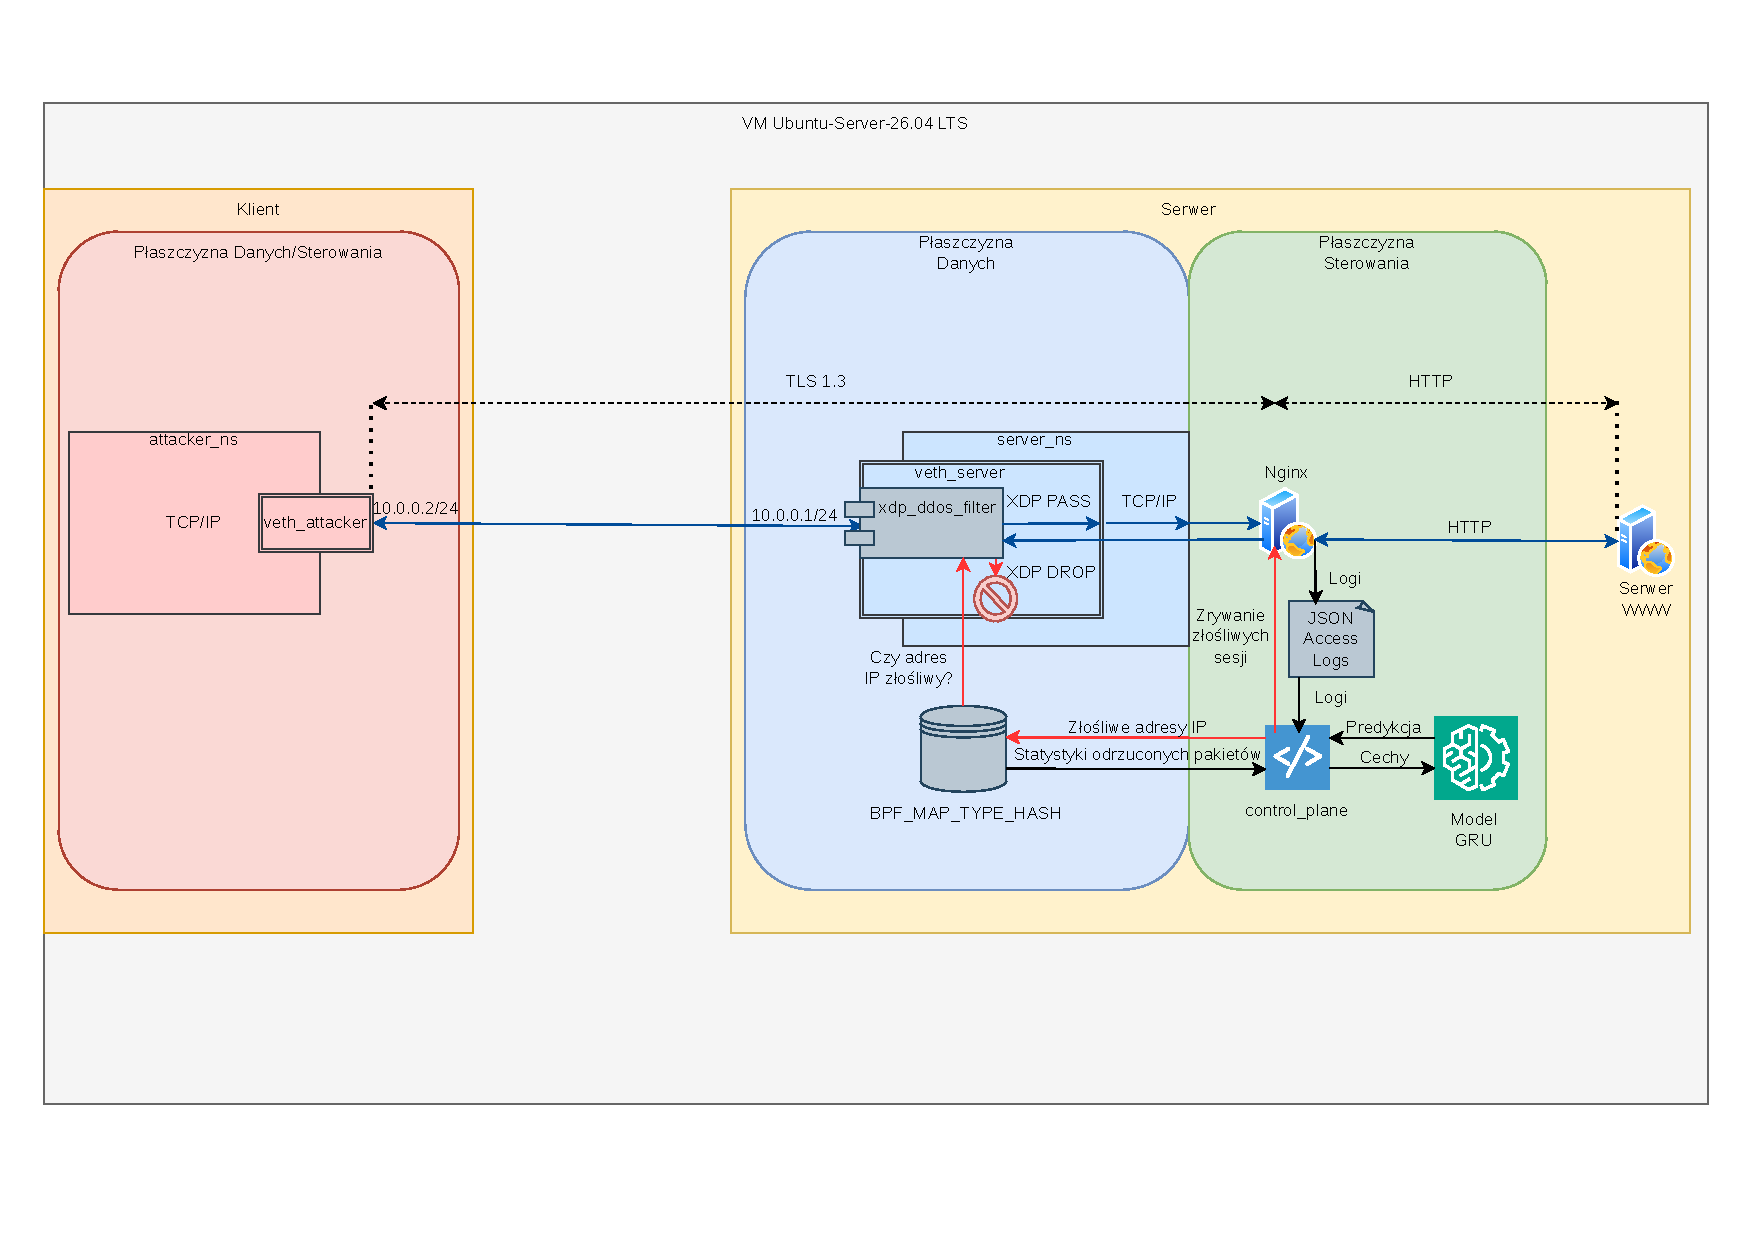
\includepdf[pages=1, landscape=true]{images/Architektura-DDoS-mitigation.pdf}
\subsection{Komponenty zastosowane w projekcie}
\begin{itemize}
    \item Środowisko sieciowe i generator ruchu: Dwie odizolowane logicznie przestrzenie nazw sieciowych (\textit{attacker\_ns} oraz \textit{server\_ns}) połączone parą wirtualnych interfejsów (\textit{veth\_attacker} i \textit{veth\_server}). Przestrzeń atakującego pozwala na generowanie sekwencji żądań HTTP o niskiej częstotliwości, symulujących zachowanie botnetu w atakach typu low-and-slow.
    
    \item Filtr płaszczyzny danych XDP/eBPF: Program niskopoziomowy w języku C \textit{xdp\_ddos\_filter.c} uruchamiany bezpośrednio na poziomie sterownika wirtualnej karty sieciowej. Odpowiada za natychmiastową ekstrakcję źródłowego adresu IP z nagłówków pakietów IPv4, weryfikację jego obecności w mapie blokad oraz wykonywanie akcji \textit{XDP\_DROP} - odrzucenie przed alokacją struktur jądra \textit{sk\_buff}, lub \textit{XDP\_PASS} - przepuszczenie pakietu do stosu TCP/IP hosta.
    
    \item Współdzielona struktura tablic eBPF Map: Zoptymalizowana mapa typu \\\textit{BPF\_MAP\_TYPE\_HASH} o nazwie \textit{blacklist\_map}, stanowiąca most pamięciowy pomiędzy przestrzenią jądra a przestrzenią użytkownika. Przechowuje zablokowane adresy IP oraz liczniki telemetrii odrzuconego ruchu, gwarantując czas wyszukiwania na poziomie $O(1)$.
    
    \item Serwer odwrotnego proxy Nginx: Komponent odpowiedzialny za zakańczanie połączeń szyfrowanych  oraz izolację właściwego serwera aplikacyjnego. Konfiguracja serwera wymusza generowanie ustrukturyzowanych logów dostępowych w formacie JSON, zawierających kluczowe metryki czasowo-rozmiarowe żądań dla modelu uczenia maszynowego.
    
    \item Model uczenia maszynowego GRU: Predykcyjna, głęboka sieć rekurencyjna zaimplementowana w bibliotece PyTorch. Model analizuje sekwencje logów sieciowych w przesuwnych oknach czasowych na podstawie trzech wyekstrahowanych cech: czasu trwania żądania, rozmiaru nagłówków oraz liczby przesłanych bajtów, klasyfikując sesje jako anomalie lub ruch prawidłowy.
    
    \item Demon integrujący w przestrzeni użytkownika: Skrypt zarządzający \textit{control\_plane.py} napisany w języku Python z wykorzystaniem biblioteki \textit{bcc}. Odpowiada za dynamiczną kompilację i załadowanie kodu XDP, asynchroniczne strumieniowanie logów z serwera Nginx, podawanie cech na wejście modelu GRU oraz realizację dwutorowej mitygacji (wstrzykiwanie IP do mapy eBPF oraz natychmiastowe zrywanie sesji TCP za pomocą narzędzia \textit{ss}).
\end{itemize}

\subsection{Szczegóły implementacji}
\begin{lstlisting}[language=Python, caption=control\_plane.py ]
from bcc import BPF
import time
import socket
import struct
import json
import os
import subprocess
from collections import defaultdict, deque
import torch
import joblib
import numpy as np
from GRU_ML_model import GRUDDoSClassifier

INTERFACE = "veth_server"
BPF_SOURCE_FILE = "xdp_ddos_filter.c"
NGINX_LOG_FILE = "/var/log/nginx/ddos_ml_access.log"
MODEL_PATH = "training_results/gru_ddos_model.pth"
SCALER_PATH = "training_results/scaler.save"

SEQUENCE_LENGTH = 15
PREDICTION_THRESHOLD = 0.85

print(f"[*] Compiling and loading eBPF code from file: {BPF_SOURCE_FILE}...")
bpf = BPF(src_file=BPF_SOURCE_FILE)
bpf_function = bpf.load_func("xdp_ddos_mitigation", BPF.XDP)
bpf.attach_xdp(INTERFACE, bpf_function, 0)
print(f"[+] Successfully attached XDP program to interface {INTERFACE}.")

blacklist_map = bpf.get_table("blacklist_map")

INPUT_SIZE = 3
HIDDEN_SIZE = 64
NUM_LAYERS = 2

print("[*] Loading data scaler...")
scaler = joblib.load(SCALER_PATH)

print("[*] Loading trained GRU model...")
device = torch.device('cuda' if torch.cuda.is_available() else 'cpu')
gru_model = GRUDDoSClassifier(input_size=INPUT_SIZE, hidden_size=HIDDEN_SIZE, num_layers=NUM_LAYERS)

gru_model.load_state_dict(torch.load(MODEL_PATH, map_location=device))
gru_model.to(device)
gru_model.eval()

def ip_to_network_bytes(ip_str):
    return struct.unpack("=I", socket.inet_aton(ip_str))[0]


def block_ip_in_xdp(ip_str):
    ip_int = ip_to_network_bytes(ip_str)
    blacklist_map[blacklist_map.Key(ip_int)] = blacklist_map.Leaf(0)
    print(f"[XDP] BLOCKED IP: {ip_str}. Rule is active on hardware.")


def kill_zombie_connections(ip_str):
    try:
        subprocess.run(["ss", "-K", "dst", ip_str], check=True, capture_output=True)
        print(f"[OS] Killed hanging TCP sessions for address {ip_str}.")
    except subprocess.CalledProcessError as e:
        print(f"[-] Error while killing sessions for {ip_str}: {e.stderr.decode().strip()}")
    except FileNotFoundError:
        print("[-] The 'ss' tool is not installed (iproute2 package).")


def tail_nginx_logs(file_path):
    with open(file_path, 'r') as f:
        f.seek(0, os.SEEK_END)
        while True:
            line = f.readline()
            if not line:
                time.sleep(0.05)
                continue
            yield line


client_sequences = defaultdict(lambda: deque(maxlen=SEQUENCE_LENGTH))
banned_ips = set()

try:
    print("[*] Starting Nginx -> GRU -> XDP integration...")
    print(f"[*] Listening for logs in file: {NGINX_LOG_FILE}")

    for log_line in tail_nginx_logs(NGINX_LOG_FILE):
        try:
            log_data = json.loads(log_line)
            client_ip = log_data.get("client_ip")

            if client_ip in banned_ips:
                continue

            features = [
                float(log_data.get("request_time", 0.0)) * 1000000,
                float(log_data.get("request_length", 0)),
                float(log_data.get("bytes_sent", 0))
            ]

            client_sequences[client_ip].append(features)

            if len(client_sequences[client_ip]) == SEQUENCE_LENGTH:
                raw_sequence = np.array(list(client_sequences[client_ip]))
                scaled_sequence = scaler.transform(raw_sequence)
                tensor_seq = torch.tensor([scaled_sequence], dtype=torch.float32).to(device)

                with torch.no_grad():
                    logits = gru_model(tensor_seq)
                    probability = torch.sigmoid(logits).item()

                if probability > PREDICTION_THRESHOLD:
                    print(f"\n[GRU] DETECTED L7 ATTACK (Slowloris/DoS) - IP: {client_ip} | Confidence: {probability * 100:.1f}%")
                    block_ip_in_xdp(client_ip)
                    kill_zombie_connections(client_ip)
                    banned_ips.add(client_ip)
                    del client_sequences[client_ip]

        except json.JSONDecodeError:
            continue
        except Exception as e:
            print(f"[-] Loop error: {e}")

except KeyboardInterrupt:
    print("\n[*] Execution interrupted by user. Cleaning up environment...")
finally:
    bpf.remove_xdp(INTERFACE, 0)
    print(f"[+] XDP program detached from {INTERFACE}. Finished.")
\end{lstlisting}
\begin{lstlisting}[language=Python, caption=GRU\_ML\_model.py]
import torch
import torch.nn as nn


class GRUDDoSClassifier(nn.Module):
    """
    Gated Recurrent Unit (GRU) classifier designed for DDoS attack detection.
    
    """

    def __init__(self, input_size, hidden_size, num_layers, output_size=1, dropout_rate=0.2):
        """
        Initializes the GRUDDoSClassifier model.

        Parameters:
        -----------
        input_size : int
            The number of expected features in the input x (e.g., request time, length, bytes sent).
        hidden_size : int
            The number of features in the hidden state h of the GRU layer.
        num_layers : int
            Number of recurrent layers stacked on top of each other (Deep RNN).
        output_size : int, optional
            The number of output units. Defaults to 1 for binary classification.
        dropout_rate : float, optional
            The dropout probability for regularization between GRU layers. Defaults to 0.2.
        """
        super(GRUDDoSClassifier, self).__init__()

        self.hidden_size = hidden_size
        self.num_layers = num_layers

        self.gru = nn.GRU(
            input_size=input_size,
            hidden_size=hidden_size,
            num_layers=num_layers,
            batch_first=True,
            dropout=dropout_rate if num_layers > 1 else 0
        )

        self.dropout = nn.Dropout(dropout_rate)
        self.fc = nn.Linear(hidden_size, output_size)

    def forward(self, x):
        """
        Performs the forward pass of the model.

        Parameters:
        -----------
        x : torch.Tensor
            Input tensor of shape (batch_size, sequence_length, input_size).

        Returns:
        --------
        torch.Tensor
            Output logits of shape (batch_size, output_size).
        """
        h0 = torch.zeros(self.num_layers, x.size(0), self.hidden_size).to(x.device)

        out, _hidden = self.gru(x, h0)
        out = out[:, -1, :]
        out = self.dropout(out)
        out = self.fc(out)

        return out
\end{lstlisting}
\begin{lstlisting}[language=Python, caption=GRU\_ML\_init.py]
import torch
import torch.nn as nn
import torch.optim as optim
import pandas as pd
import numpy as np
import joblib
from sklearn.preprocessing import StandardScaler
from torch.utils.data import Dataset, DataLoader
from GRU_ML_model import GRUDDoSClassifier

DATA_PATH = "training_data/DoS1-Thursday-15-02-2018_TrafficForML_CICFlowMeter.parquet"
MODEL_SAVE_PATH = "training_results/gru_ddos_model.pth"
SCALER_SAVE_PATH = "training_results/scaler.save"

SEQUENCE_LENGTH = 15
BATCH_SIZE = 64
EPOCHS = 5
HIDDEN_SIZE = 64
NUM_LAYERS = 2

device = torch.device('cuda' if torch.cuda.is_available() else 'cpu')
print(f"[*] Using device: {device}")

print("[*] Loading .parquet data...")
df = pd.read_parquet(DATA_PATH)

df = df.iloc[:len(df)//2].reset_index(drop=True)
print(f"[*] Dataset reduced to: {len(df)} rows (chronological order preserved).")

df.replace([np.inf, -np.inf], np.nan, inplace=True)
df.dropna(inplace=True)

ip_col = 'Src IP' if 'Src IP' in df.columns else 'Source IP' if 'Source IP' in df.columns else None
time_col = 'Timestamp' if 'Timestamp' in df.columns else None

if ip_col:
    print(f"[*] Sorting data by {ip_col} to group sequences per client...")
    sort_cols = [ip_col]
    
    if time_col:
        sort_cols.append(time_col)
        # Przekształcamy Timestamp dla pewności poprawnego sortowania czasu
        df[time_col] = pd.to_datetime(df[time_col], errors='ignore')
    
    # Sortowanie zapewnia, że wszystkie pakiety z jednego IP leżą obok siebie w pamięci
    df = df.sort_values(by=sort_cols).reset_index(drop=True)
else:
    print("[-] Warning: Client IP column not found in dataset. Sequences might cross IPs!")

if 'Label' in df.columns:
    labels = np.where(df['Label'] == 'Benign', 0, 1)
else:
    raise ValueError("Missing 'Label' column in dataset!")

selected_features = [
    'Flow Duration',
    'Fwd Packets Length Total',
    'Bwd Packets Length Total'
]
features = df[selected_features]
INPUT_SIZE = features.shape[1]
print(f"[*] Detected features (INPUT_SIZE): {INPUT_SIZE}")

print("[*] Normalizing data...")
scaler = StandardScaler()
features_scaled = scaler.fit_transform(features)

joblib.dump(scaler, SCALER_SAVE_PATH)

print("[*] Generating time sequences...")


class DynamicDDoSDataset(Dataset):
    """
    Dataset class for dynamically generating time-series sequences from network traffic data.
    """
    def __init__(self, data, labels, seq_length):
        """
        Initializes the dynamic dataset.

        Parameters:
        -----------
        data : numpy.ndarray
            The scaled feature array.
        labels : numpy.ndarray
            The binary target labels.
        seq_length : int
            The number of time steps in each sequence.
        """
        self.data = data
        self.labels = labels
        self.seq_length = seq_length

    def __len__(self):
        """
        Returns the total number of available sequences.
        """
        return len(self.data) - self.seq_length

    def __getitem__(self, idx):
        """
        Generates one sequence slice and its corresponding label on the fly.
        """
        x_seq = self.data[idx : (idx + self.seq_length)]
        y_label = self.labels[idx + self.seq_length - 1]
        return torch.tensor(x_seq, dtype=torch.float32), torch.tensor([y_label], dtype=torch.float32)


print("[*] Generating dynamic loader...")
dataset = DynamicDDoSDataset(features_scaled, labels, SEQUENCE_LENGTH)
dataloader = DataLoader(dataset, batch_size=BATCH_SIZE, shuffle=True)

model = GRUDDoSClassifier(input_size=INPUT_SIZE, hidden_size=HIDDEN_SIZE, num_layers=NUM_LAYERS).to(device)
criterion = nn.BCEWithLogitsLoss()
optimizer = optim.Adam(model.parameters(), lr=0.001)

print("[*] Starting training process...")
for _epoch in range(EPOCHS):
    model.train()
    total_loss = 0
    for batch_X, batch_y in dataloader:
        batch_X, batch_y = batch_X.to(device), batch_y.to(device)

        optimizer.zero_grad()
        outputs = model(batch_X)
        loss = criterion(outputs, batch_y)
        loss.backward()
        optimizer.step()

        total_loss += loss.item()

    avg_loss = total_loss / len(dataloader)
    print(f"Epoch [{_epoch + 1}/{EPOCHS}], Loss: {avg_loss:.4f}")

torch.save(model.state_dict(), MODEL_SAVE_PATH)
print(f"[+] Model successfully saved to {MODEL_SAVE_PATH}")
print(f"[+] Scaler successfully saved to {SCALER_SAVE_PATH}")
\end{lstlisting}
\begin{lstlisting}[language=Bash, caption=setup.sh]
#!/bin/bash

PROJECT_DIR="/home/artur/DDoS-mitigation"
NGINX_CONF="${PROJECT_DIR}/nginx.conf"
CONTROL_PLANE="${PROJECT_DIR}/control_plane.py"
PYTHON_VENV="${PROJECT_DIR}/.venv/bin/python"

if [ "$EUID" -ne 0 ]; then
  echo "[-] Please run this script with root privileges (sudo bash setup_lab.sh)"
  exit
fi

echo "[*] Starting the construction of the automated PoC environment..."

echo "[*] Checking dependencies (Nginx)..."
if ! command -v nginx &> /dev/null; then
    echo "[*] Installing Nginx server..."
    apt-get update && apt-get install -y nginx
fi

systemctl stop nginx 2>/dev/null
systemctl disable nginx 2>/dev/null

echo "[*] Killing old processes from previous sessions..."
pkill -f "nginx: master process" 2>/dev/null
pkill -f "control_plane.py" 2>/dev/null
pkill -f "gunicorn" 2>/dev/null # <-- Dodane: Czyszczenie Gunicorna

ip netns del attacker_ns 2>/dev/null
ip netns del server_ns 2>/dev/null

echo "[*] Creating Network Namespaces and veth interfaces..."
ip netns add attacker_ns
ip netns add server_ns

ip link add veth_server type veth peer name veth_attacker

ip link set veth_server netns server_ns
ip link set veth_attacker netns attacker_ns

ip netns exec server_ns ip addr add 10.0.0.1/24 dev veth_server
ip netns exec server_ns ip link set veth_server up
ip netns exec server_ns ip link set lo up

ip netns exec attacker_ns ip addr add 10.0.0.2/24 dev veth_attacker
ip netns exec attacker_ns ip link set veth_attacker up
ip netns exec attacker_ns ip link set lo up

ip netns exec server_ns ethtool -K veth_server tx off rx off

echo "[+] Built network environment: [10.0.0.1 Server] <- veth -> [10.0.0.2 Attacker]"

echo "[*] Preparing logs and SSL certificates for Proxy..."

if [ ! -f /etc/ssl/certs/nginx-selfsigned.crt ]; then
    openssl req -x509 -nodes -days 365 -newkey rsa:2048 \
        -keyout /etc/ssl/private/nginx-selfsigned.key \
        -out /etc/ssl/certs/nginx-selfsigned.crt \
        -subj "/C=PL/ST=Masovian/L=Warsaw/O=PoC/CN=twojadomena.pl" 2>/dev/null
fi

mkdir -p /var/log/nginx
touch /var/log/nginx/ddos_ml_access.log
chmod 644 /var/log/nginx/ddos_ml_access.log
> /var/log/nginx/ddos_ml_access.log

echo "[*] Creating a robust dummy backend app..."
cat << 'EOF' > ${PROJECT_DIR}/dummy_app.py
def app(environ, start_response):
    data = b"Backend is running flawlessly!\n"
    start_response("200 OK", [
        ("Content-Type", "text/plain"),
        ("Content-Length", str(len(data)))
    ])
    return iter([data])
EOF

echo "[*] Installing Gunicorn inside venv..."
${PYTHON_VENV} -m pip install gunicorn >/dev/null 2>&1

echo "[*] Starting multi-worker Gunicorn backend on port 8080..."
ip netns exec server_ns nohup ${PYTHON_VENV} -m gunicorn --chdir ${PROJECT_DIR} --workers 4 --threads 10 -b 0.0.0.0:8080 dummy_app:app >/dev/null 2>&1 &

echo "[*] Starting Nginx in isolated namespace..."
ip netns exec server_ns nginx -c ${NGINX_CONF}

echo "------------------------------------------------------------"
echo "[+] Infrastructure ready! Starting Mitigation Daemon."
echo "------------------------------------------------------------"

ip netns exec server_ns ${PYTHON_VENV} ${CONTROL_PLANE}
\end{lstlisting}
\begin{lstlisting}[language=C, caption=xdp\_ddos\_filter.c]
#include <uapi/linux/bpf.h>
#include <uapi/linux/if_ether.h>
#include <uapi/linux/ip.h>
#include <uapi/linux/in.h>

BPF_HASH(blacklist_map, u32, u64, 100000);

int xdp_ddos_mitigation(struct xdp_md *ctx) {
    void *data_end = (void *)(long)ctx->data_end;
    void *data     = (void *)(long)ctx->data;

    struct ethhdr *eth = data;

    if ((void *)(eth + 1) > data_end) {
        return XDP_PASS;
    }

    if (eth->h_proto != bpf_htons(ETH_P_IP)) {
        return XDP_PASS;
    }

    struct iphdr *ip = data + sizeof(*eth);

    if ((void *)(ip + 1) > data_end) {
        return XDP_PASS;
    }

    u32 src_ip = ip->saddr;

    u64 *drop_counter = blacklist_map.lookup(&src_ip);

    if (drop_counter) {
        lock_xadd(drop_counter, 1);
        return XDP_DROP;
    }

    return XDP_PASS;
}
\end{lstlisting}
\begin{lstlisting}[language=conf, caption=nginx.conf]
worker_processes auto;
worker_rlimit_nofile 65535;
events {
    worker_connections 16384;
    use epoll;
    multi_accept on;
}
http {
    limit_req_zone $binary_remote_addr zone=mylimit:10m rate=20r/s;
    log_format json_ml_format escape=json
    '{'
        '"timestamp":"$time_iso8601",'
        '"client_ip":"$remote_addr",'
        '"request_method":"$request_method",'
        '"request_uri":"$request_uri",'
        '"status":$status,'
        '"request_time":$request_time,'
        '"request_length":$request_length,'
        '"bytes_sent":$bytes_sent,'
        '"user_agent":"$http_user_agent"'
    '}';

    access_log /var/log/nginx/ddos_ml_access.log json_ml_format;
    error_log /var/log/nginx/error.log warn;

    client_body_timeout 10s;
    client_header_timeout 10s;
    keepalive_timeout 15s;
    send_timeout 10s;

    client_max_body_size 2M;
    large_client_header_buffers 2 1k;

    server {
        listen 80;
        listen 443 ssl http2;
        server_name twojadomena.pl localhost;

        ssl_certificate /etc/ssl/certs/nginx-selfsigned.crt;
        ssl_certificate_key /etc/ssl/private/nginx-selfsigned.key;

        ssl_protocols TLSv1.2 TLSv1.3;
        ssl_prefer_server_ciphers on;

        location / {
            limit_req zone=mylimit burst=100 nodelay;
            proxy_pass http://127.0.0.1:8080;

            proxy_set_header Host $host;
            proxy_set_header X-Real-IP $remote_addr;
            proxy_set_header X-Forwarded-For $proxy_add_x_forwarded_for;
            proxy_set_header X-Forwarded-Proto $scheme;

            proxy_connect_timeout 5s;
            proxy_send_timeout 10s;
            proxy_read_timeout 10s;
        }
    }
}
\end{lstlisting}
\section{Przeprowadzenie testów opracowanego systemu}
\section{Ocena uzyskanych wyników}
\section{Wnioski}
\begin{thebibliography}{9}
\bibitem{Detecting and Mitigating DDoS Attacks with AI: A Survey}
\href{https://arxiv.org/html/2503.17867v1#bib.bib96}{Detecting and Mitigating DDoS Attacks with AI: A Survey}
\bibitem{SYN flood DDoS attack - Cloudflare}
\href{https://www.cloudflare.com/pl-pl/learning/ddos/syn-flood-ddos-attack/}{SYN flood DDoS attack - Cloudflare}
\bibitem{DDoS Protection and Mitigation: A 2026 Guide to Defending Modern Networks}
\href{https://www.kentik.com/kentipedia/ddos-protection/}{DDoS Protection and Mitigation: A 2026 Guide to Defending Modern Networks}
\bibitem{DNS amplification attack}
\href{https://www.cloudflare.com/pl-pl/learning/ddos/dns-amplification-ddos-attack/}{DNS amplification attack}
\bibitem{Slowloris DDoS attack}
\href{https://www.cloudflare.com/pl-pl/learning/ddos/ddos-attack-tools/slowloris/}{Slowloris DDoS attack}
\bibitem{Slowloris attack}
\href{https://www.invicti.com/learn/slowloris-attack}{Slowloris attack}
\bibitem{Generator of Slow Denial-of-Service Cyber Attacks}
\href{https://pmc.ncbi.nlm.nih.gov/articles/PMC8401215/}{Generator of Slow Denial-of-Service Cyber Attacks}
\bibitem{CVE-2023-44487}
\href{https://nvd.nist.gov/vuln/detail/cve-2023-44487}{CVE-2023-44487}
\bibitem{HTTP/2 Rapid Reset: deconstructing the record-breaking attack}
\href{https://blog.cloudflare.com/technical-breakdown-http2-rapid-reset-ddos-attack/}{HTTP/2 Rapid Reset: deconstructing the record-breaking attack}

\bibitem{How Cloudflare auto-mitigated world record 3.8 Tbps DDoS attack}
\href{https://blog.cloudflare.com/how-cloudflare-auto-mitigated-world-record-3-8-tbps-ddos-attack/}{How Cloudflare auto-mitigated world record 3.8 Tbps DDoS attack}

\bibitem{How to Set Up Rate Limiting with iptables to Prevent DDoS}
\href{https://oneuptime.com/blog/post/2026-03-20-iptables-rate-limiting-ddos/view}{How to Set Up Rate Limiting with iptables to Prevent DDoS}

\bibitem{Building a High-Performance DDoS Mitigation Pipeline with nftables and XDP}
\href{https://dev.to/arzenlabscom/building-a-high-performance-ddos-mitigation-pipeline-with-nftables-and-xdp-2e0j}{Building a High-Performance DDoS Mitigation Pipeline with nftables and XDP}

\bibitem{How to use eBPF XDP for DDoS protection at network edge}
\href{https://oneuptime.com/blog/post/2026-02-09-ebpf-xdp-ddos-protection/view}{How to use eBPF XDP for DDoS protection at network edge}

\bibitem{Anycast}
\href{https://en.wikipedia.org/wiki/Anycast}{Anycast}

\bibitem{Top F5 Alternatives for WAF in 2026}
\href{https://www.indusface.com/blog/f5-waf-alternatives/}{Top F5 Alternatives for WAF in 2026}

\bibitem{Linux ACL
Performance Analysis}
\href{https://netdevconf.info/0x15/slides/7/LinuxACLPerformanceAnalysis.pdf}{Linux ACL
Performance Analysis}

\bibitem{Cloud-based DDoS detection using hybrid feature selection with deep reinforcement learning (DRL)}
\href{https://pmc.ncbi.nlm.nih.gov/articles/PMC12540699/}{Cloud-based DDoS detection using hybrid feature selection with deep reinforcement learning (DRL)}

\bibitem{Enhanced DDoS Attack Detection Using Advanced Deep Learning Techniques}
\href{https://ieeexplore.ieee.org/document/10829087}{Enhanced DDoS Attack Detection Using Advanced Deep Learning Techniques}

\bibitem{collaborative-p4-sdn-ddos-detection-and-mitigation-with-early-exit-neural-networks}
\href{https://www.themoonlight.io/es/review/collaborative-p4-sdn-ddos-detection-and-mitigation-with-early-exit-neural-networks}{collaborative-p4-sdn-ddos-detection-and-mitigation-with-early-exit-neural-networks}

\bibitem{Carpet-bombing Attacks Highlight the Need for Intelligent and Automated DDoS Protection}
\href{https://www.a10networks.com/blog/carpet-bombing-attacks-highlight-the-need-for-intelligent-and-automated-ddos-protection/}{Carpet-bombing Attacks Highlight the Need for Intelligent and Automated DDoS Protection}

\bibitem{The ultimate weapon against DDoS — BGP Flowspec}
\href{https://blog.apnic.net/2024/09/18/the-ultimate-weapon-against-ddos-bgp-flowspec/}{The ultimate weapon against DDoS — BGP Flowspec}

\end{thebibliography}
\end{document}
